\chapter*{Préface}

\textit{Voici le manuel d'utilisation officiel de ToM+, rédigé à la main par moi-même (Fabio Java) en anglais, sans recourir à
aucun outil d'IA, ni dans ce guide ni dans le code qui permet à ToM+ de fonctionner. Les autres langues
que l'anglais ont été traduites automatiquement à l'aide de} \href{https://www.deepl.com/en/translator}
    {DeepL}.\\

\textit{À l'ère de la génération automatisée de contenu, ce manuel se distingue et vous pouvez
être assuré que toutes les fonctionnalités proposées ainsi que l'interface utilisateur ont été rédigées par un être humain.
C’est ce qui rend ce projet unique parmi toutes les alternatives : savoir exactement
ce que fait le code est essentiel pour développer consciemment de nouvelles fonctionnalités, corriger les bugs et
garantir une assistance aux autres utilisateurs de ToM+ si nécessaire.}\\

\textit{ToM+ évolue constamment grâce à sa vaste communauté issue du
} \href{https://www.twizy-forum.de/twiz-o-meter}
    {forum allemand consacré à la Twizy}. \textit{Si vous 
souhaitez vous procurer un exemplaire de ToM+, envoyez-moi un e-mail à l’adresse} \textbf{info.twizometer@gmail.com}.
\textit{Si vous souhaitez proposer une nouvelle fonctionnalité, signaler un bug ou même une faute de frappe dans ce
manuel, veuillez m’envoyer un e-mail ou ouvrir une pull request sur} \href{https://codeberg.org/fabio-java/ToM-Wizard}
    {Codeberg}.\\

\textit{Si vous possédez un ToM standard ou un BigToM, vous pouvez également vous référer à ce manuel d’utilisation,
car les fonctionnalités sont fondamentalement les mêmes, à l’exception du ToM standard qui ne dispose pas
de la page du tableau de bord ni des pages de recharge en 3D.}\\

\textit{Le ToM n’est pas un produit commercial et il est fabriqué à la main par un amateur comme moi ; chaque 
unité est unique et doit être considérée comme un prototype, sans logo CE ni aucun autre 
test officiel. Le Twiz O'meter lit les données du bus CAN sans nécessiter aucune
modification du véhicule, mais je décline toute responsabilité quant à son installation
et à son utilisation.}\\

\textit{Ce manuel d’utilisation est mis à jour pour la version 2.4 du micrologiciel ESP.}


\chapter{Description et liste des fonctionnalités}

\section{ToM+ : points forts}

ToM+ dispose de nombreuses fonctions et peut être mis à jour en permanence au fur et à mesure du
développement du micrologiciel. Dans les paragraphes suivants, je vais vous présenter brièvement ses
fonctionnalités, afin de vous donner une idée du type de produit que j’expliquerai plus loin dans ce manuel.

\subsection{Un nouveau tableau de bord pour la Twizy}

Étant donné que le tableau de bord de notre Twizy n’affiche que quelques valeurs, telles que la vitesse et les
kilomètres restants, j’ai décidé de développer cet écran très pratique, qui affichera bien
plus de données, en les lisant directement à partir du bus CAN de la Twizy, via le connecteur OBD
situé dans la boîte à gants gauche. ToM se contentera de « capter » les valeurs transmises par la Twizy, puis de
les afficher sur l’écran LCD, ce qui permettra de nombreuses autres fonctionnalités. ToM dispose d’une mémoire minuscule
mais puissante, capable de stocker certaines de ces valeurs pendant la conduite afin de vous fournir
un historique de vos trajets. Sa capacité à stocker certaines valeurs permet de
sauvegarder vos configurations et personnalisations sur le ToM, même après une mise à jour du micrologiciel.

\begin{figure}[H]
    \centering
    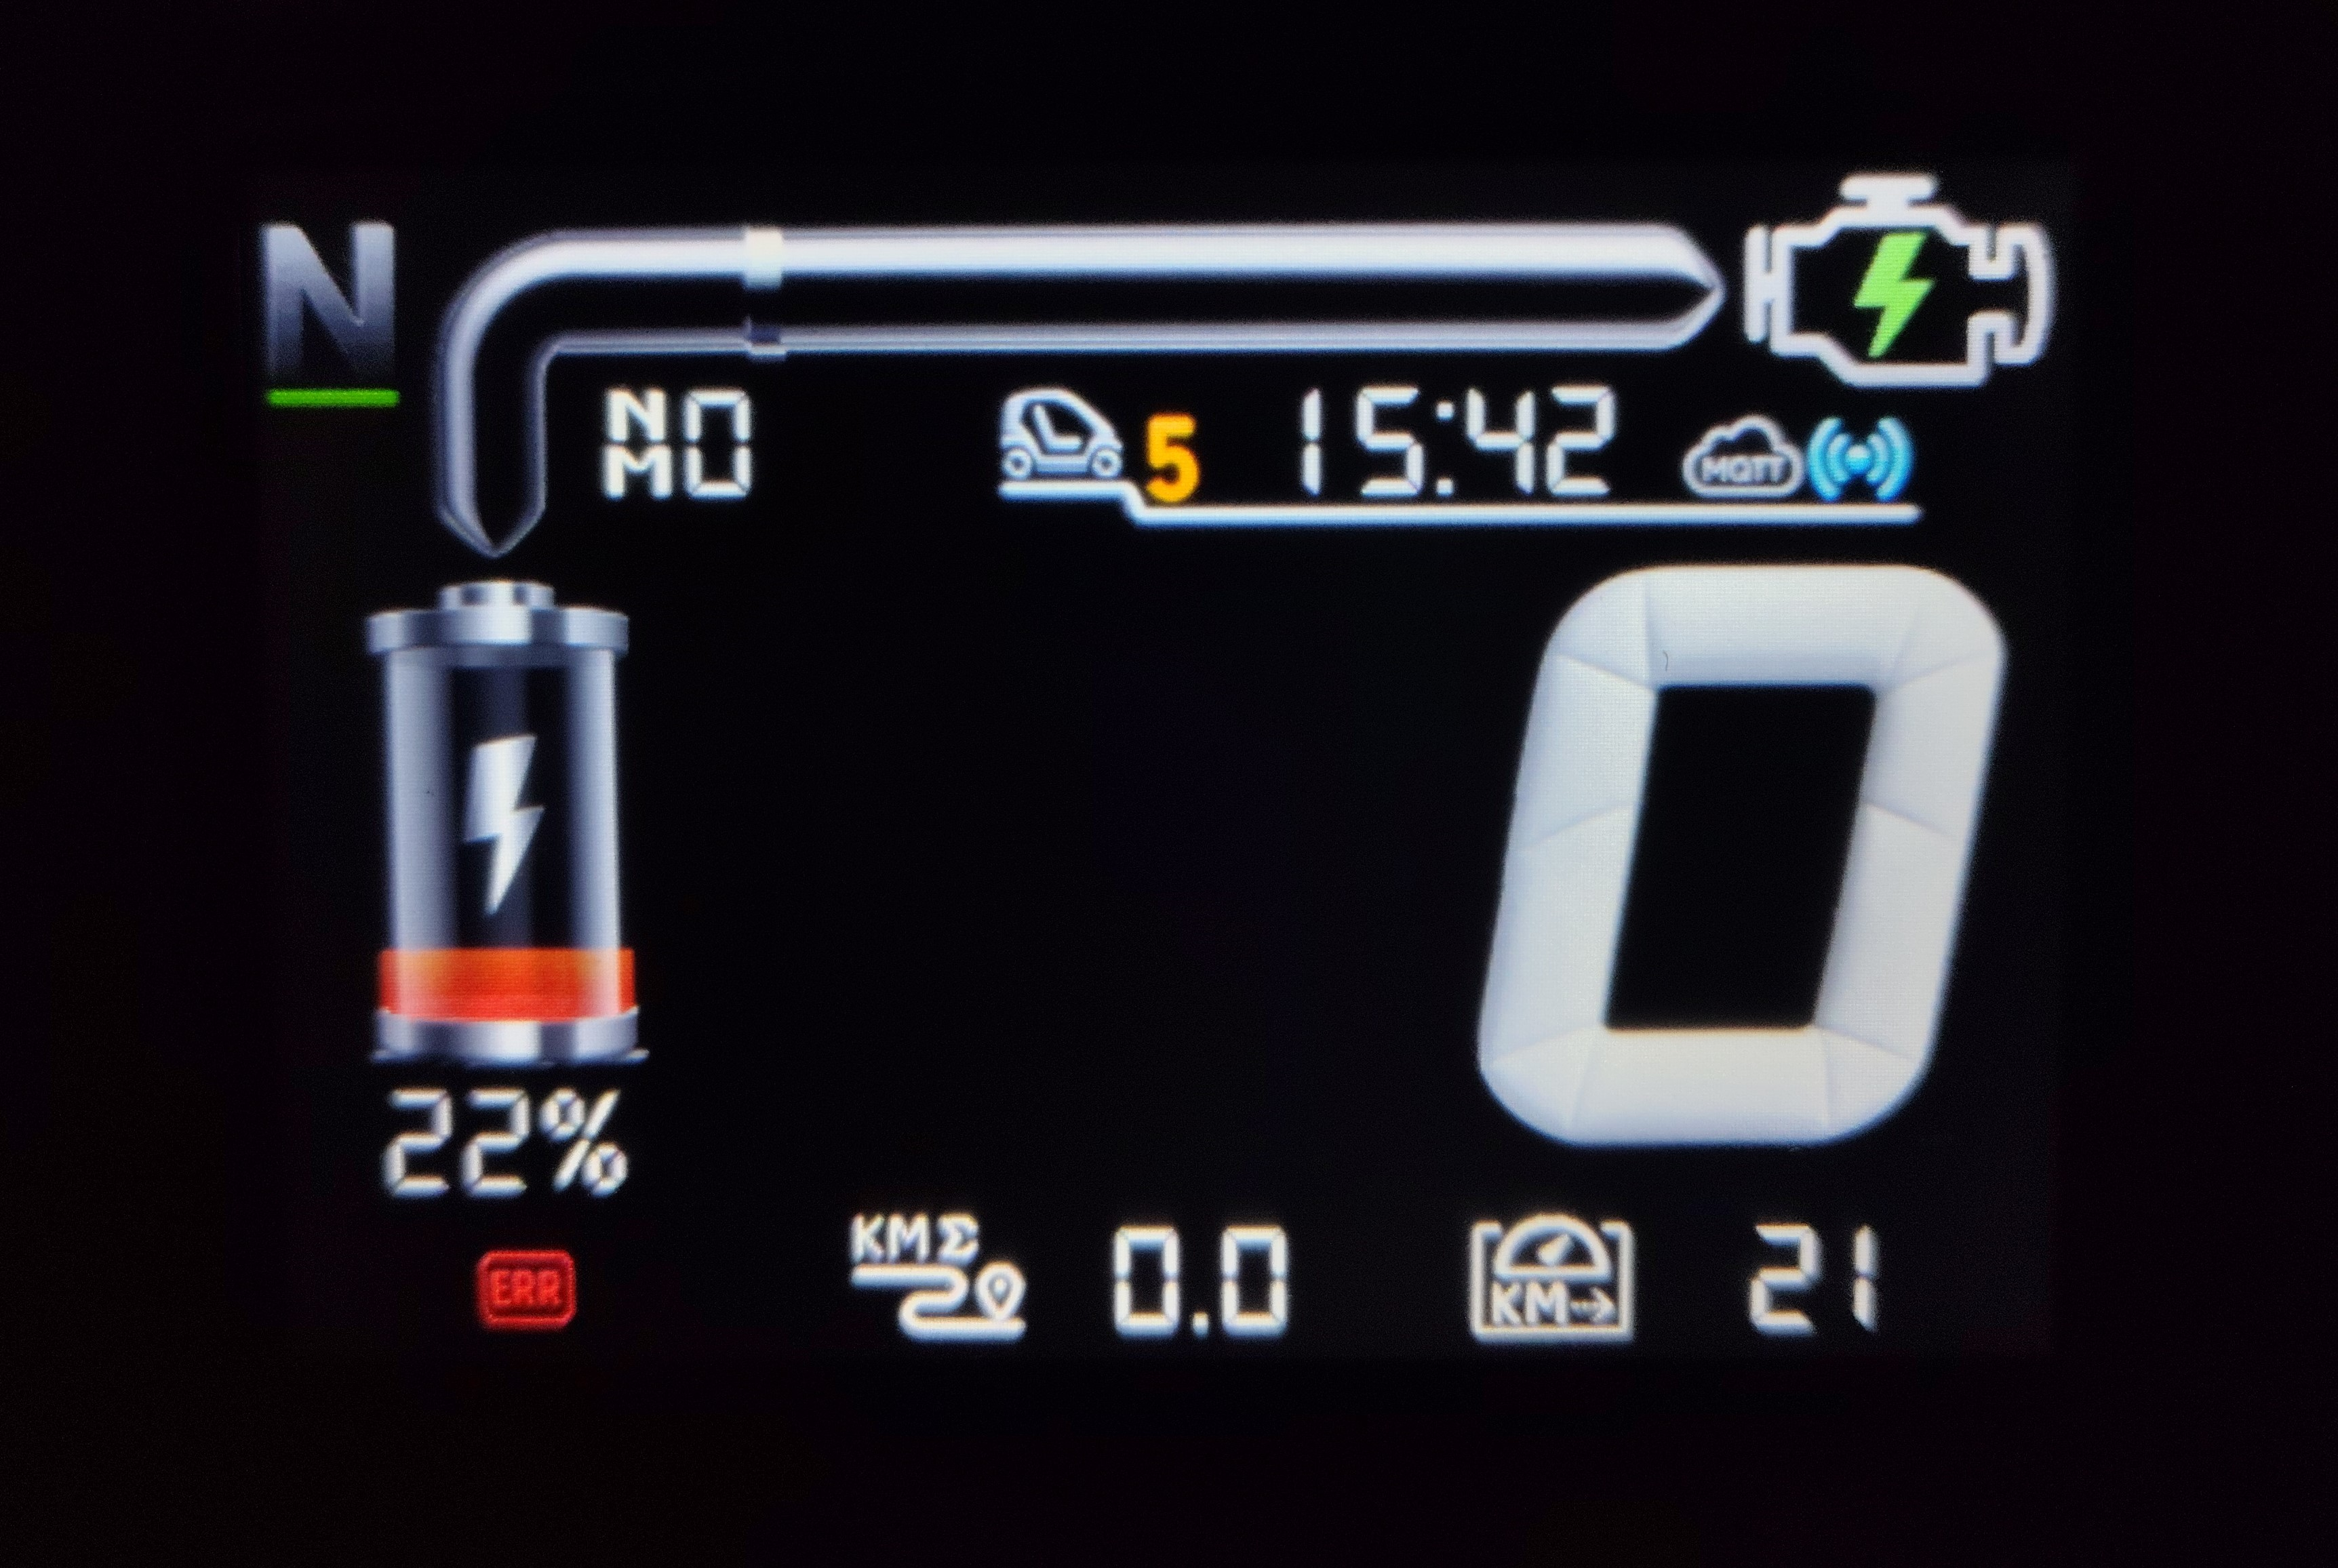
\includegraphics[width=0.8\textwidth]{figures/dashboard.jpg}
    \caption{Tableau de bord du ToM+}
\end{figure}

Il s'efforce de conserver le même style que le tableau de bord d'origine de la Twizy, mais avec un aspect plus moderne et
en 3D.
Comme sur le tableau de bord d’origine, vous disposez des informations suivantes : la batterie, le rapport engagé, l’autonomie restante en kilomètres, la vitesse et l’heure.
Mais j’ai ajouté le \textbf{pourcentage exact de charge de la batterie}, le couple moteur, quelques icônes d’état, des informations sur le trajet et bien d’autres éléments que vous pouvez configurer à votre guise et que nous verrons en détail plus tard.

La page principale est personnalisable et vous pouvez choisir ce qui y est affiché, tout comme les autres pages que vous pouvez parcourir à l’aide du bouton que vous pouvez monter sur la tige d’essuie-glace.
L’aspect général des autres pages est illustré sur l’image, avec une valeur au premier plan et les autres sur le côté gauche. En bas
, vous pouvez changer de page en appuyant sur son icône.

\begin{figure}[H]
    \centering
    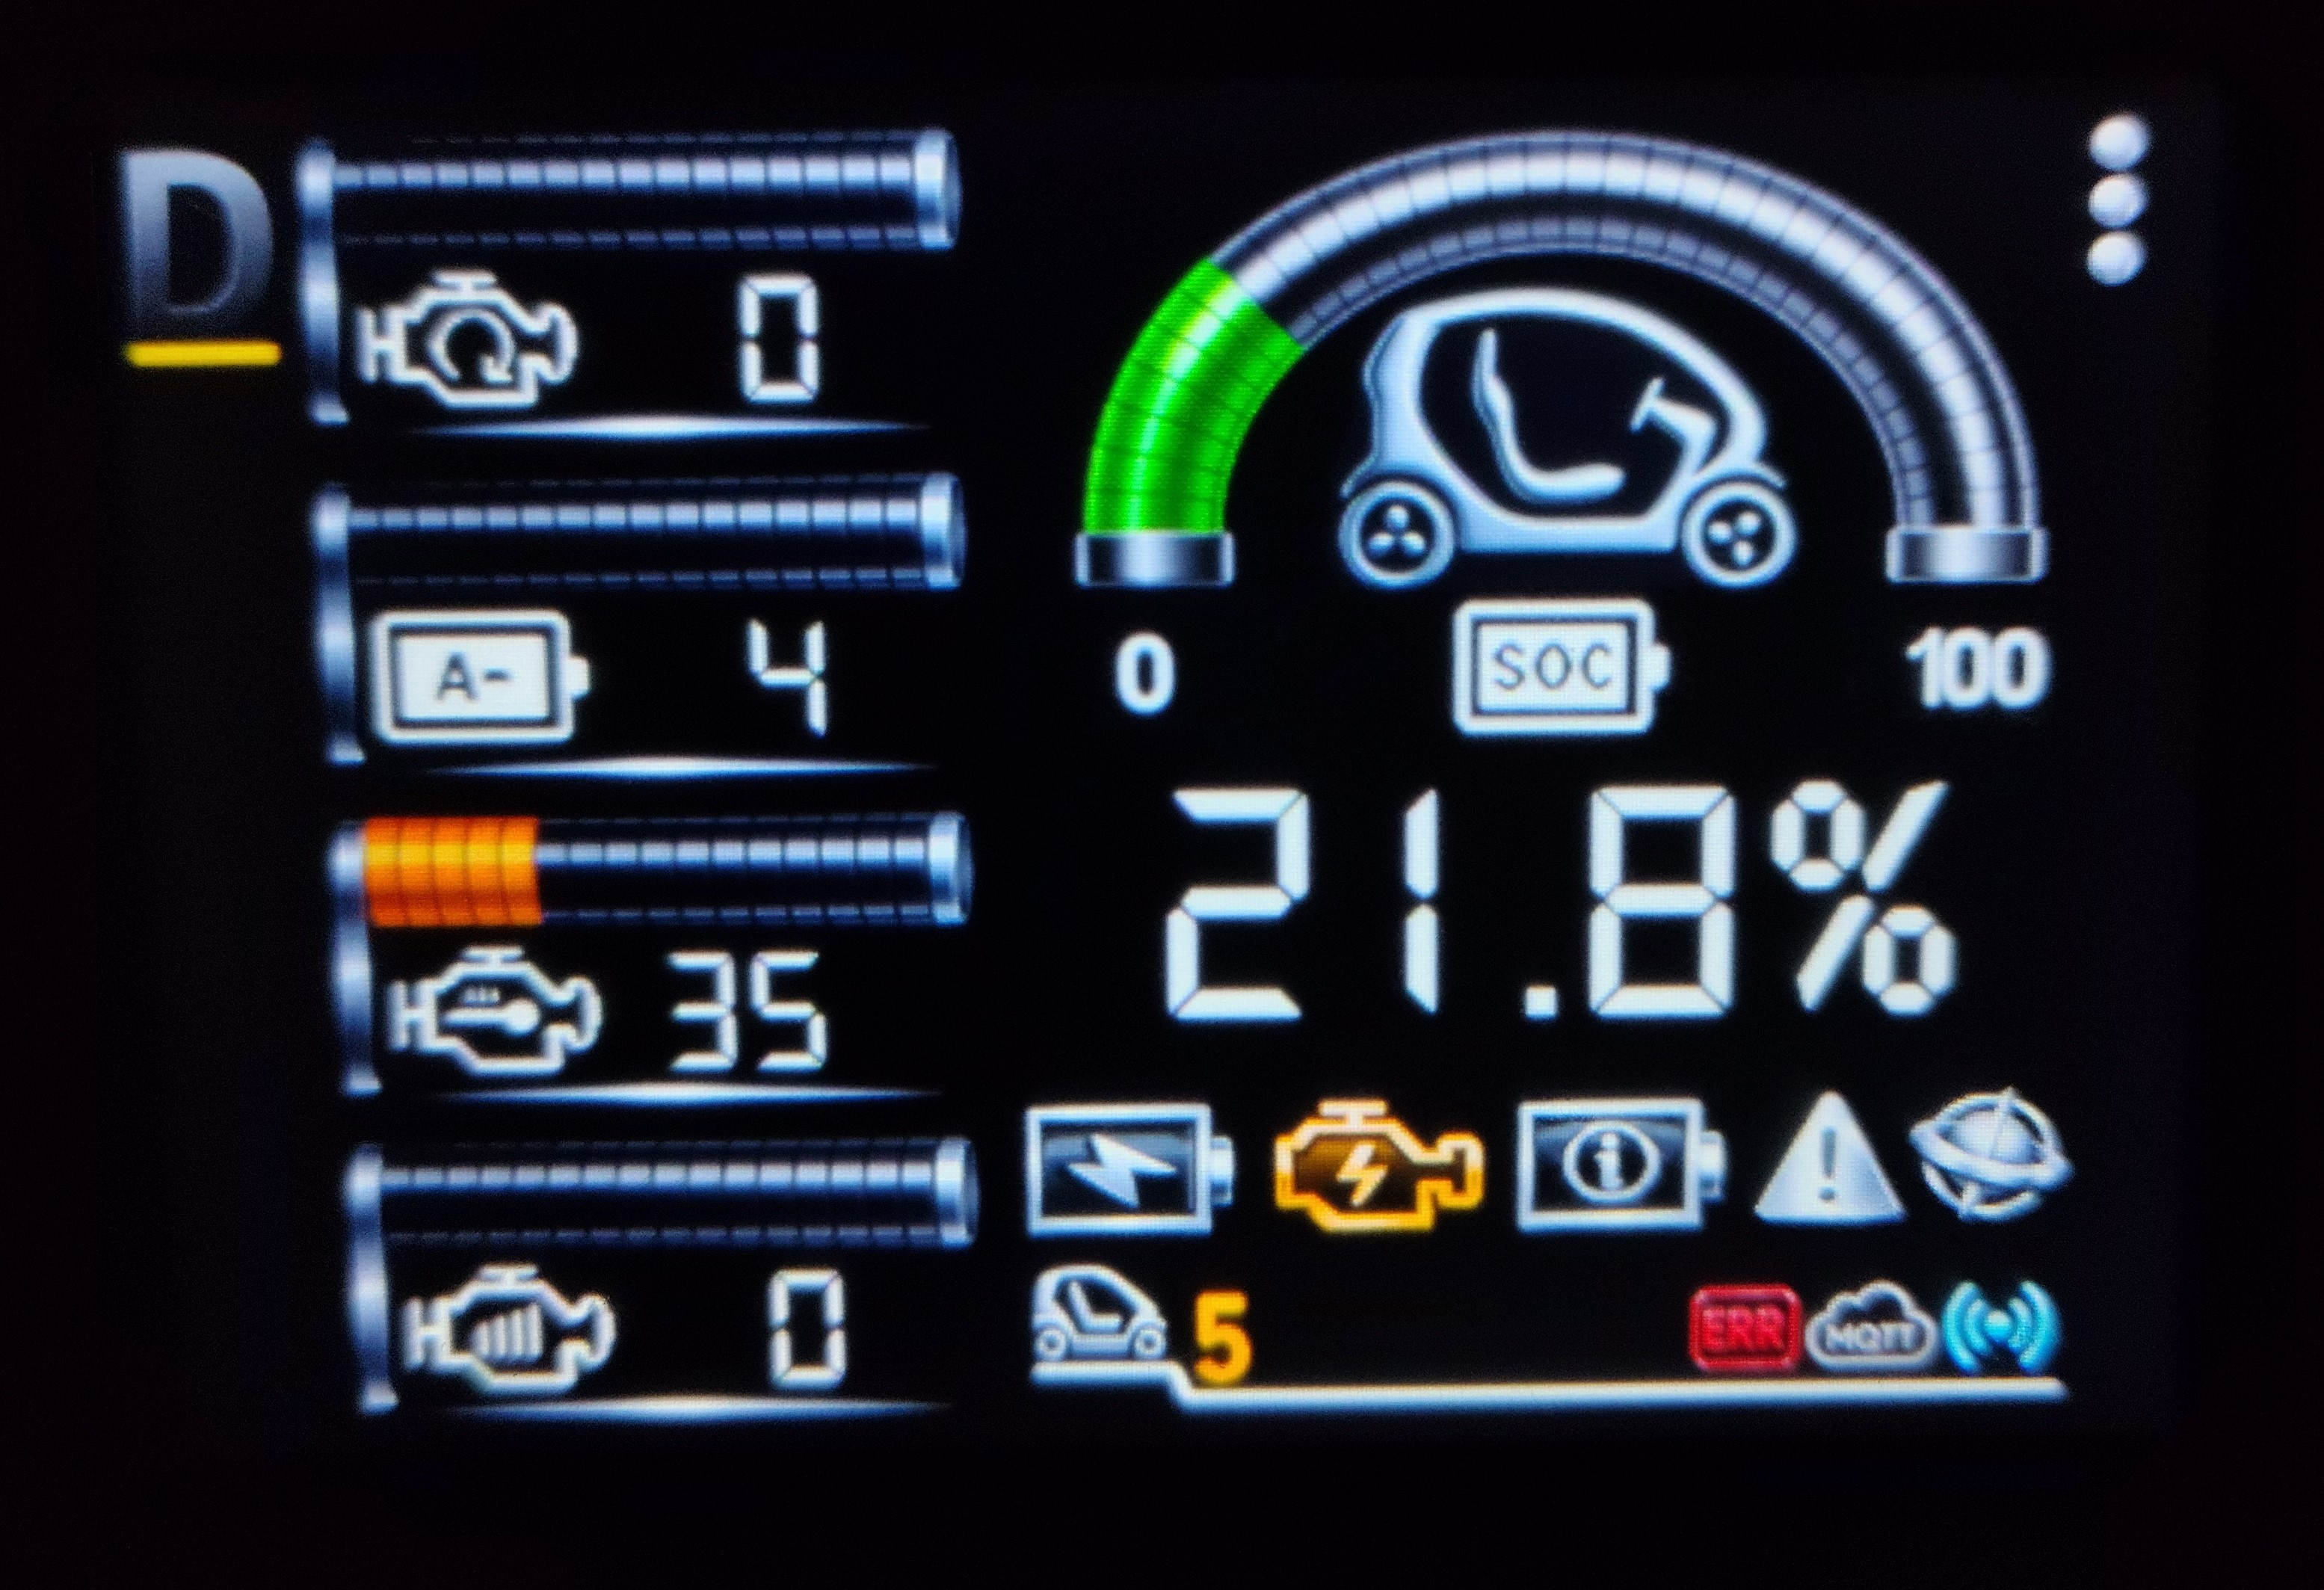
\includegraphics[width=0.8\textwidth]{figures/engine_page.jpg}
    \caption{Page « Moteur » du ToM+}
\end{figure}

\subsection{Connectivité Wi-Fi}

La carte ESP32 contenue dans le boîtier noir permet de se connecter à un
point d’accès réseau Wi-Fi. Une fois le ToM+ connecté, de nombreuses possibilités s’offrent à vous. Par
exemple, cet appareil peut être utilisé pour transférer des données de votre Twizy vers votre \textbf{MQTT}
, où vous pourrez utiliser ces données pour intégrer votre voiture à votre système domotique IoT. 

Ce n’est pas la seule fonctionnalité liée à la connexion Wi-Fi dont dispose le ToM+. Il peut également 
faire office de point d’accès grâce à son SSID et à son mot de passe, créant ainsi un réseau privé sans 
connexion à Internet. De cette manière, vous pouvez vous connecter en toute sécurité, \textbf{en acceptant de maintenir le profil de connexion}
actif même s’il ne fournit aucune connexion à Internet (un message d’avertissement s’affiche généralement sur les
téléphones Android 10 secondes après la première connexion), puis effectuer vos
configurations supplémentaires sur certaines pages web hébergées par ToM+ lui-même. Il vous suffit de saisir
dans votre navigateur préféré l’adresse IPv4 privée statique de ToM (\textbf{\textit{192.188.1.188}}) et profitez-en !

\begin{figure}[H]
    \centering
    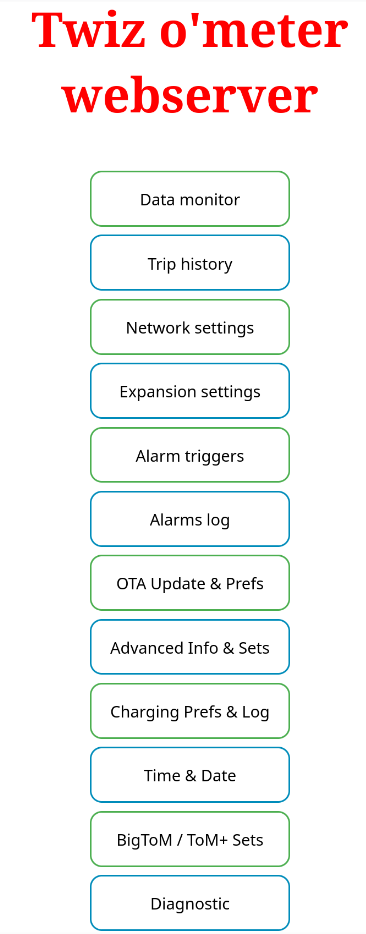
\includegraphics[
        width=\textwidth,
        height=0.75\textheight,
        keepaspectratio
    ]{figures/landing_page.png}
    
    \caption{Page d’accueil du serveur web}
\end{figure}

Comme vous pouvez le constater dans cette nouvelle version de ToM, le serveur web est bien plus complet et convivial. Vous pouvez facilement naviguer parmi les pages et configurer votre appareil comme vous le souhaitez. Le serveur web est également adaptatif, ce qui vous permet de l’utiliser également sur votre smartphone ou votre tablette.

\subsection{Application mobile ToM}

Parallèlement aux mises à jour du micrologiciel de l’écran LCD et de la boîte noire, une application Android minimaliste est
également mise à jour et vous permettra de surveiller les données en temps réel de votre Twizy à l’aide
de votre smartphone. 

La mise en page s’efforce d’imiter l’interface graphique d’origine de ToM et s’appuie sur le protocole \textbf{MQTT} pour partager
et transférer les valeurs de ToM+ vers l’application ; vous devrez donc la configurer à la fois
sur l’application et sur la page MQTT de ToM+, en inversant les rubriques IN et OUT. L’application est
distribuée sous la forme d’un fichier \textbf{APK}, un programme d’installation pour applications Android qui
vous permet d’installer cette application même sans connexion Internet. Elle est disponible \href{https://www.mediafire.com/file/du7px1bzq0zzdxu/TwizOMeter_v3.1.2.apk/file}
    {en cliquant ici}.

Vous devrez peut-être activer l’option « Installer des applications provenant de sources inconnues » dans les paramètres de votre téléphone pour ouvrir un fichier
portant l’extension \textit{(.apk)}. Au premier démarrage, vous verrez peut-être apparaître une fenêtre contextuelle indiquant que cette application
a été créée pour une version plus ancienne d’Android si vous disposez d’un téléphone plus récent : cliquez simplement sur OK
et ignorez ce message (l’application fonctionnera parfaitement). Voici un aperçu de la page de chargement et des paramètres de l’application :

\begin{figure}[H]
    \centering
    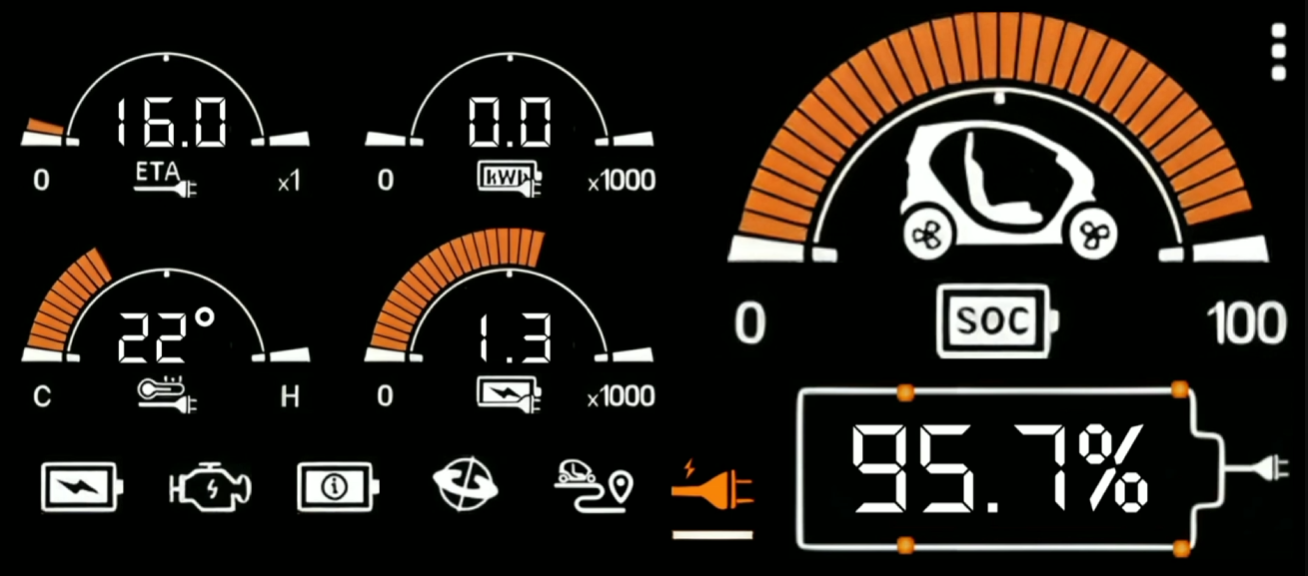
\includegraphics[width=0.8\textwidth]{figures/tom_app_charging.png}
    \caption{Page de recharge de l’application Android ToM+}
\end{figure}

\begin{figure}[H]
    \centering
    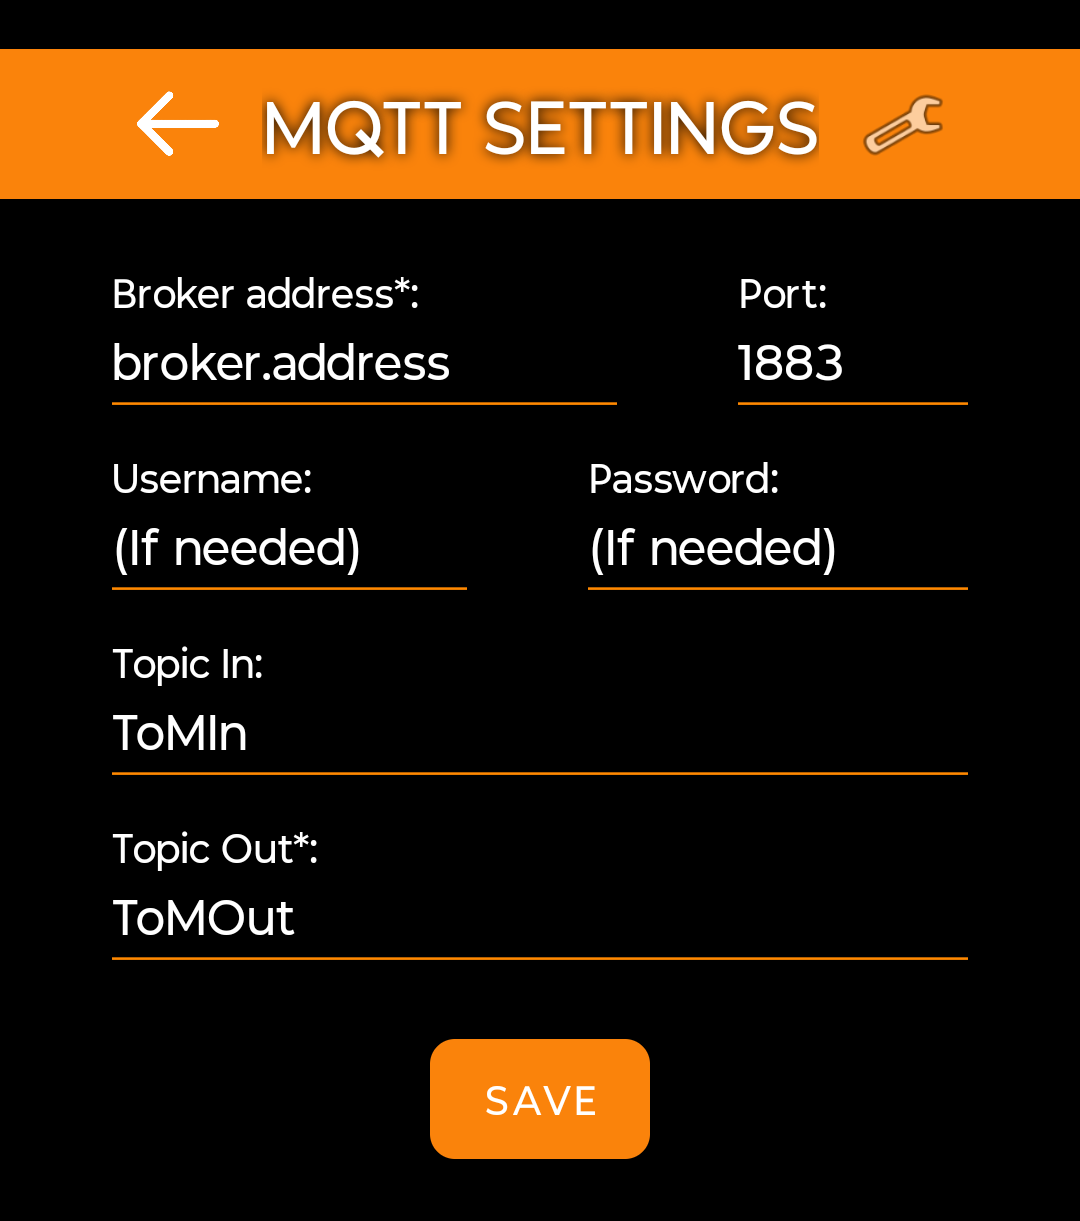
\includegraphics[width=0.65\textwidth]{figures/tom_app_settings.png}
    \caption{Page des paramètres de l’application Android ToM+}
\end{figure}

\subsection{Bref aperçu de la consommation}

ToM utilise l’alimentation par batterie 12 V, prélevée directement sur le connecteur OBD, et
ne consomme pas beaucoup, comme le montrent les mesures progressives ci-dessous.

\begin{figure}[H]
    \centering
    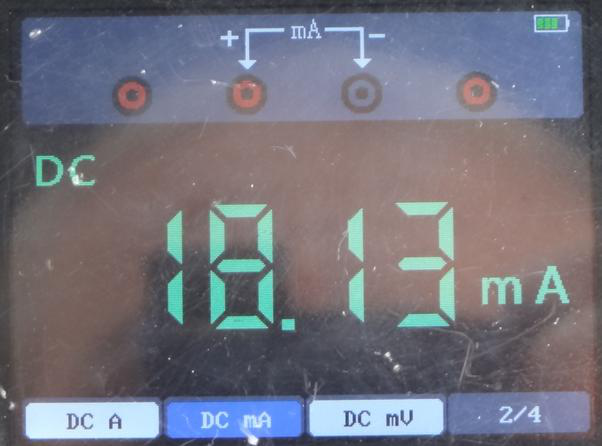
\includegraphics[width=0.65\textwidth]{figures/consumption_off.png}
    \caption{Consommation lorsque la Twizy est à l’arrêt}
\end{figure}

Lorsque la carte mère est active et que l’écran est allumé, la consommation est d’environ 90 mA. Si le Wi-Fi est également activé, la consommation électrique est proche de celle indiquée ci-dessous (peut-être légèrement supérieure en raison des dernières mises à jour qui ont introduit les graphismes 3D).

\begin{figure}[H]
    \centering
    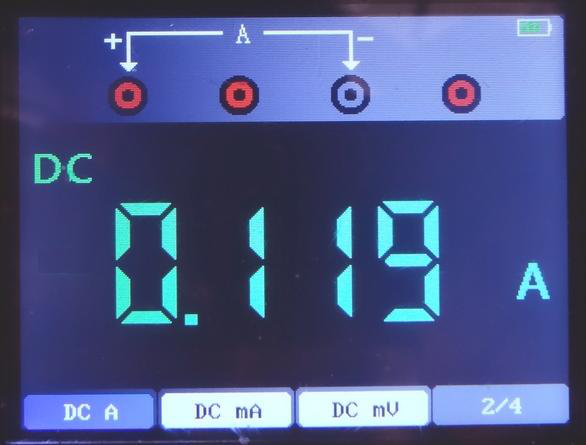
\includegraphics[width=0.65\textwidth]{figures/consumption_on_wifi.png}
    \caption{Consommation lorsque le ToM+ est activé avec le Wi-Fi}
\end{figure}

Lorsque le Twizy est éteint, le boîtier noir passe en mode veille et consomme 18 mA.
De plus, la fonction tactile vous permettra d’interagir beaucoup plus facilement avec l’
appareil et son écran LCD. Comme il utilise une technologie tactile résistive, vous pouvez utiliser  vos
 doigts ou un petit stylet en plastique dur pour appuyer sur les boutons. Ce n’est pas aussi performant que
  les tableaux de bord à écran tactile capacitif, mais une fois que vous l’aurez essayé, vous ne pourrez plus vous en passer, 
  croyez-moi !

\clearpage

\section{Kit ToM+ fourni}

Lorsque le ToM+ est expédié, il est généralement emballé dans une boîte marron afin de protéger les cartes électroniques internes
et les capteurs des chocs pendant le transport. Dans cette nouvelle version, plus besoin de longs câbles : un seul câble plus court est relié à la carte mère interne du ToM+, logée dans un petit boîtier en plastique noir
que j’appelle généralement la « boîte noire ». Bien sûr, l’écran tactile LCD résistif est également fourni, sur lequel vous pouvez visualiser et configurer tous les paramètres.
Plus besoin de vis ni de ruban adhésif ! Il suffit d’un simple clip permettant de fixer l’écran directement sur le tableau de bord d’origine.

\begin{figure}[H]
    \centering
    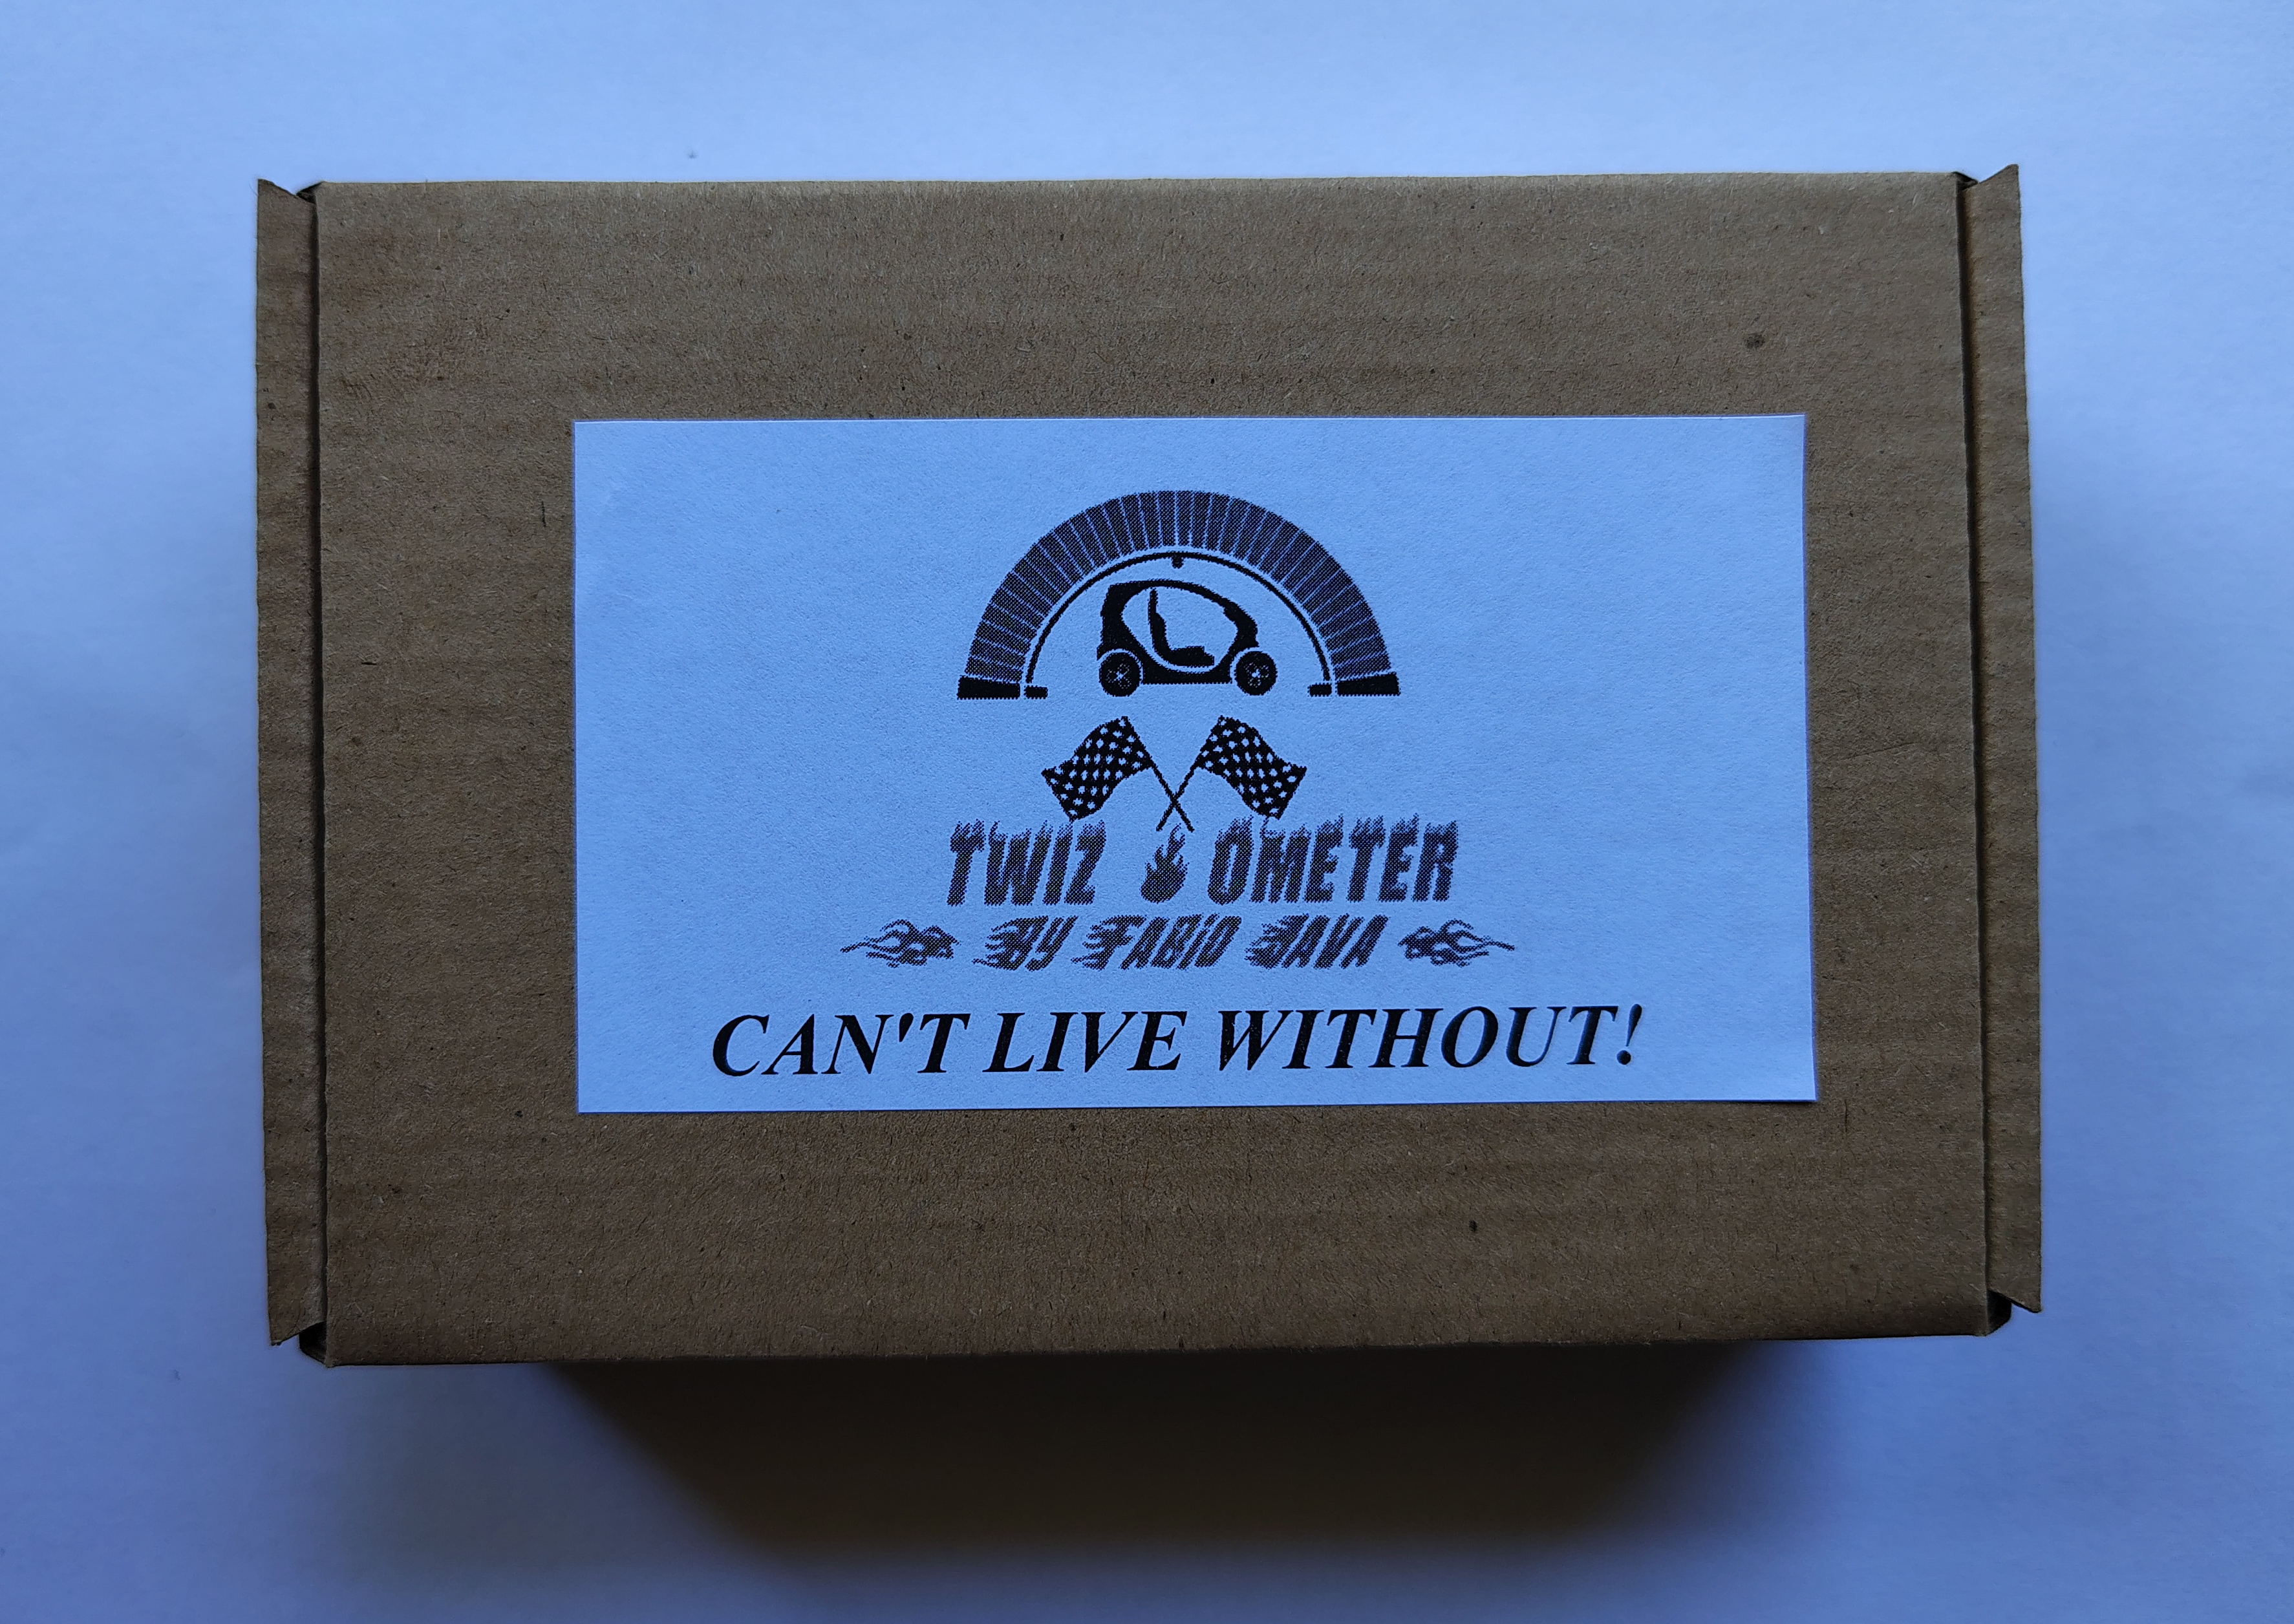
\includegraphics[width=0.8\textwidth]{figures/box.png}
    \caption{Kit ToM+ fourni}
\end{figure}

\subsection{La « boîte noire »}

La « boîte noire » est la carte mère du ToM+ et contient la plupart des composants nécessaires
au fonctionnement du système. Elle offre :
\begin{itemize}
    \item Un connecteur externe pour l’écran LCD ;
    \item Un connecteur d’extension avec des broches d’alimentation et GPIO ;
    \item Un port OBD femelle intégré pour le bus CAN de la Twizy ;
    \item Un port microUSB pour les mises à jour du micrologiciel ;
    \item Un connecteur femelle pour le bouton situé sur la manette d’essuie-glace ;
    \item Un interrupteur marche/arrêt ToM+
\end{itemize}

\begin{figure}[H]
    \centering
    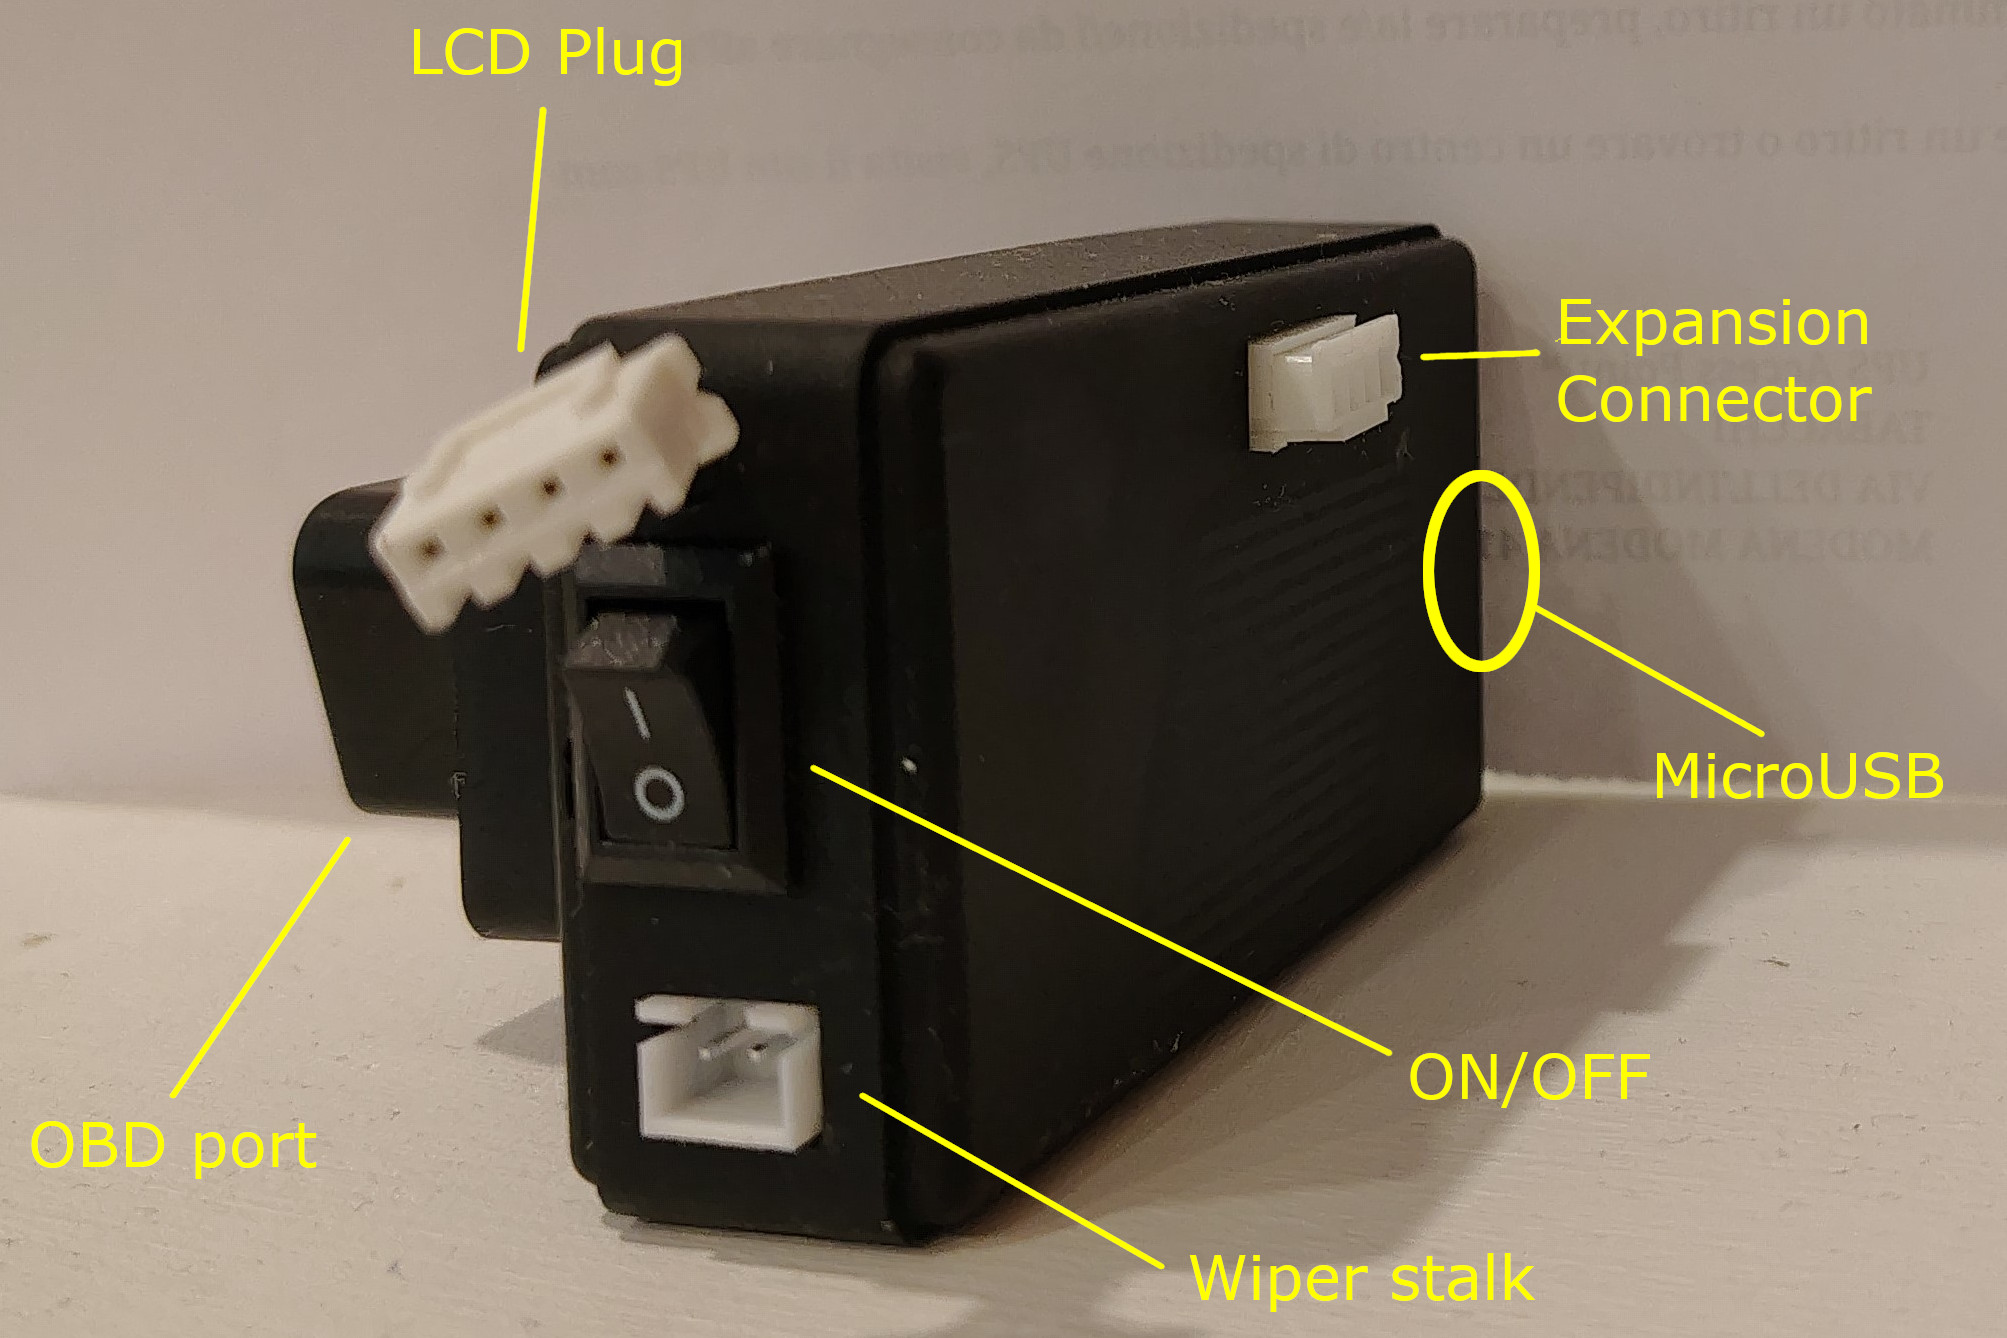
\includegraphics[width=0.75\textwidth]{figures/black_box.jpg}
    \caption{Le boîtier noir}\label{fig:blackbox_components}
    \end{figure}

\subsection{Le connecteur d’extension}

Si vous souhaitez personnaliser davantage votre ToM+, vous pouvez facilement le faire à l’aide du connecteur
illustré sur l’image ci-contre. En effet, il fournit une alimentation supplémentaire de 5 V provenant de
VCC (ancien câble rouge) et de la masse (GND) (ancien câble noir), ce qui vous permet d’alimenter une LED externe, un
petit buzzer ou tout autre dispositif de votre choix. Les deux autres câbles sont des broches d’entrée-sortie générales,
la broche 1 (câble jaune) et la broche 2 (câble bleu). Elles peuvent remplir des fonctions d’entrée ou de sortie, selon votre choix sur la \textit{« page d’extension »} du serveur web ToM \textbf{.} Dans cette dernière version de l’appareil, le connecteur d’extension est intégré au boîtier noir (sans câbles colorés), mais le brochage reste identique.
N’oubliez pas de retirer le capot de protection avant de l’utiliser et de vous limiter à une tension d’entrée de \textbf{3,3 V maximum}. Pour des tensions plus élevées,
prévoyez un diviseur de tension adapté.

\begin{figure}[H]
    \centering
    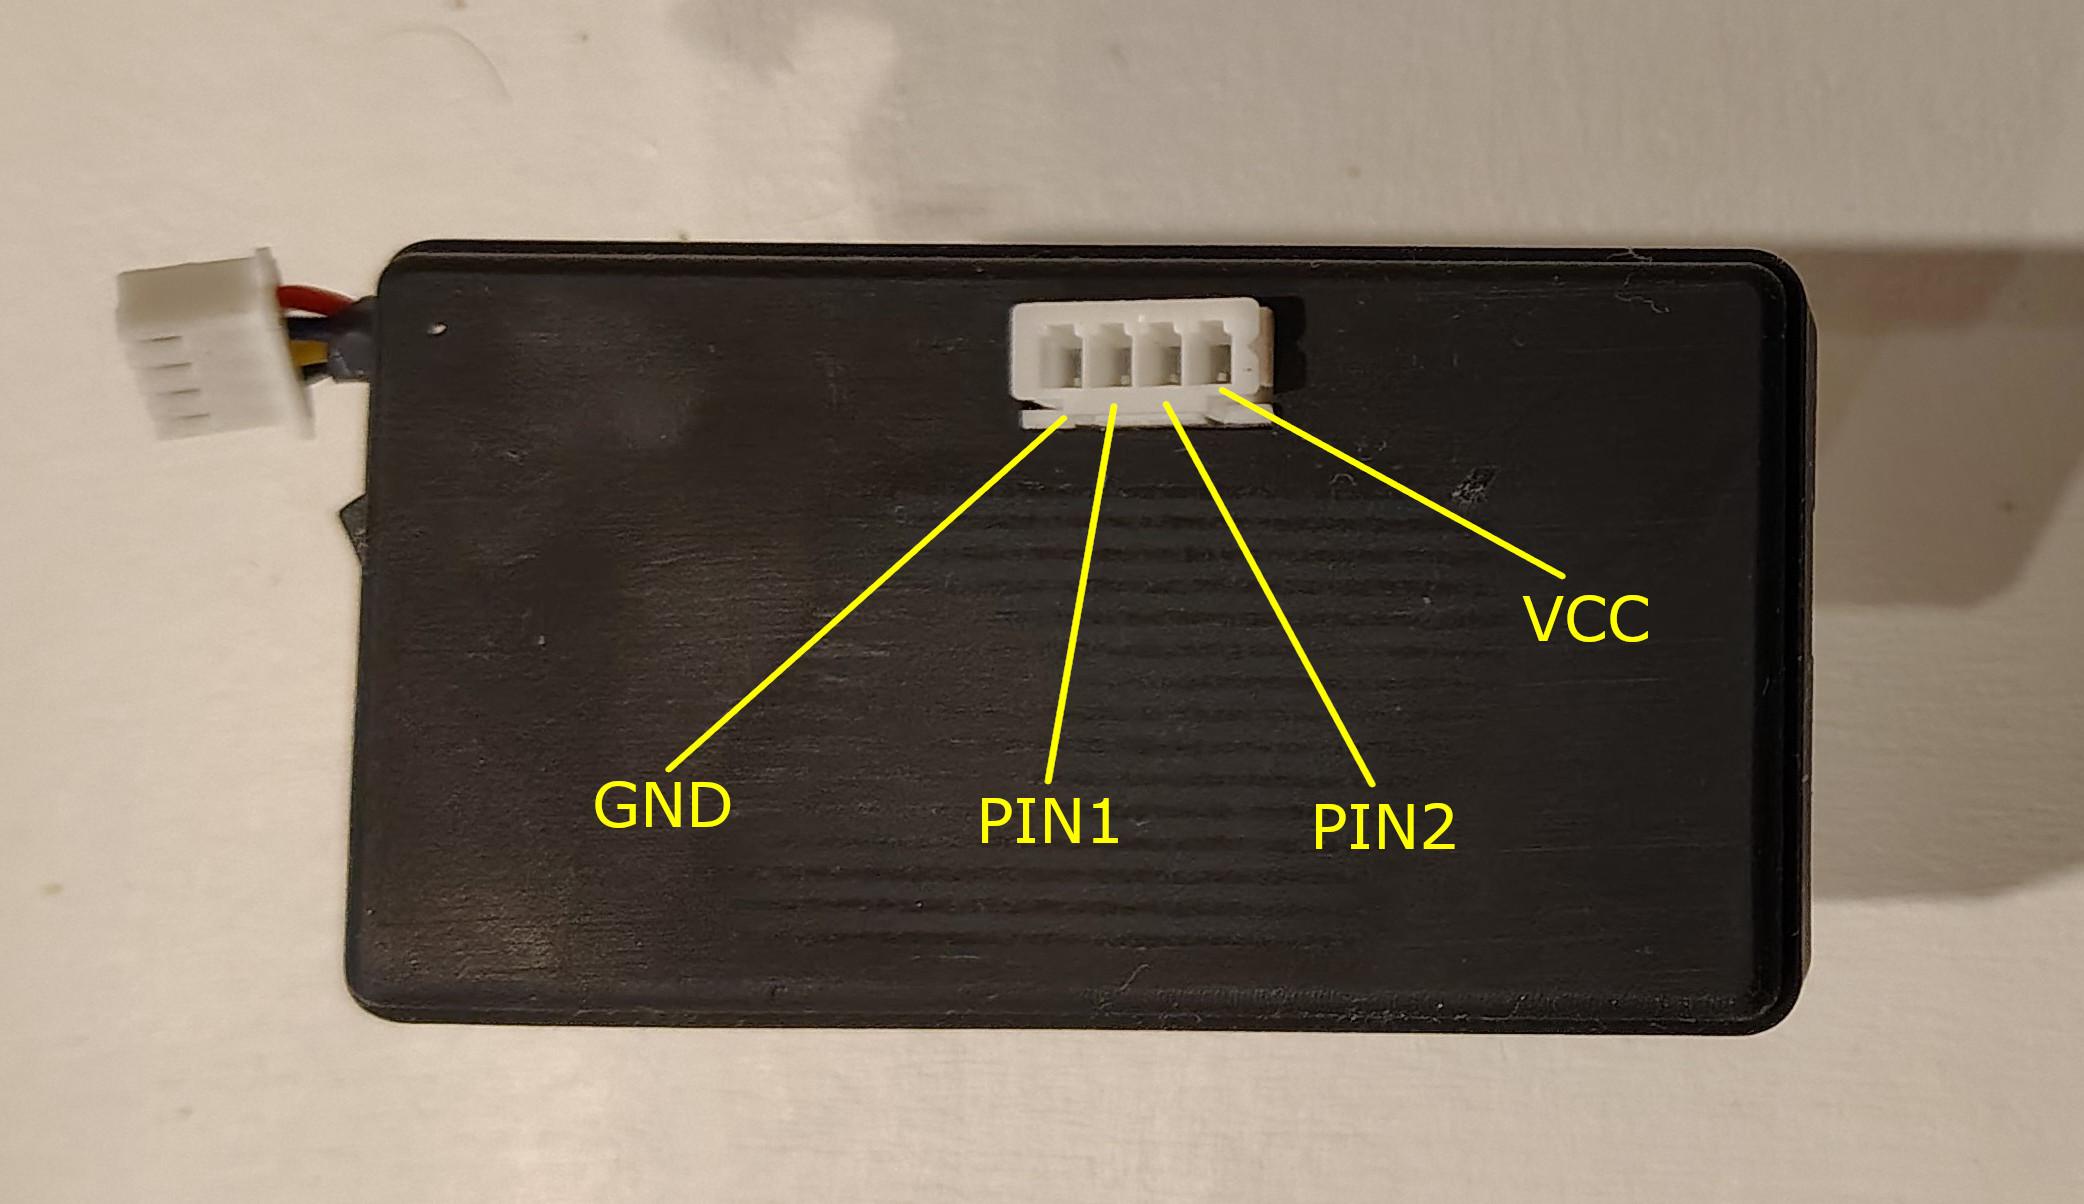
\includegraphics[width=0.7\textwidth]{figures/expansion_bb.jpg}
    \caption{Connecteur d’extension}\label{fig:expansion_pinout}
    \end{figure}

\subsection{L’écran LCD et son support}

L’écran LCD tactile résistif est intégré dans un support imprimé en 3D qui se fixe sur le tableau de bord d’origine. Si vous le souhaitez, vous pouvez également disposer d’un support autonome imprimé en 3D pour monter l’écran sur la boîte à gants, à l’instar du ToM standard. Vous disposez ainsi d’un appareil 2 en 1 pouvant être utilisé aussi bien en version à clipser qu’en version autonome, selon vos préférences. Un emplacement pour carte microSD est accessible pour les mises à jour du micrologiciel.

\begin{figure}[H]
    \centering
    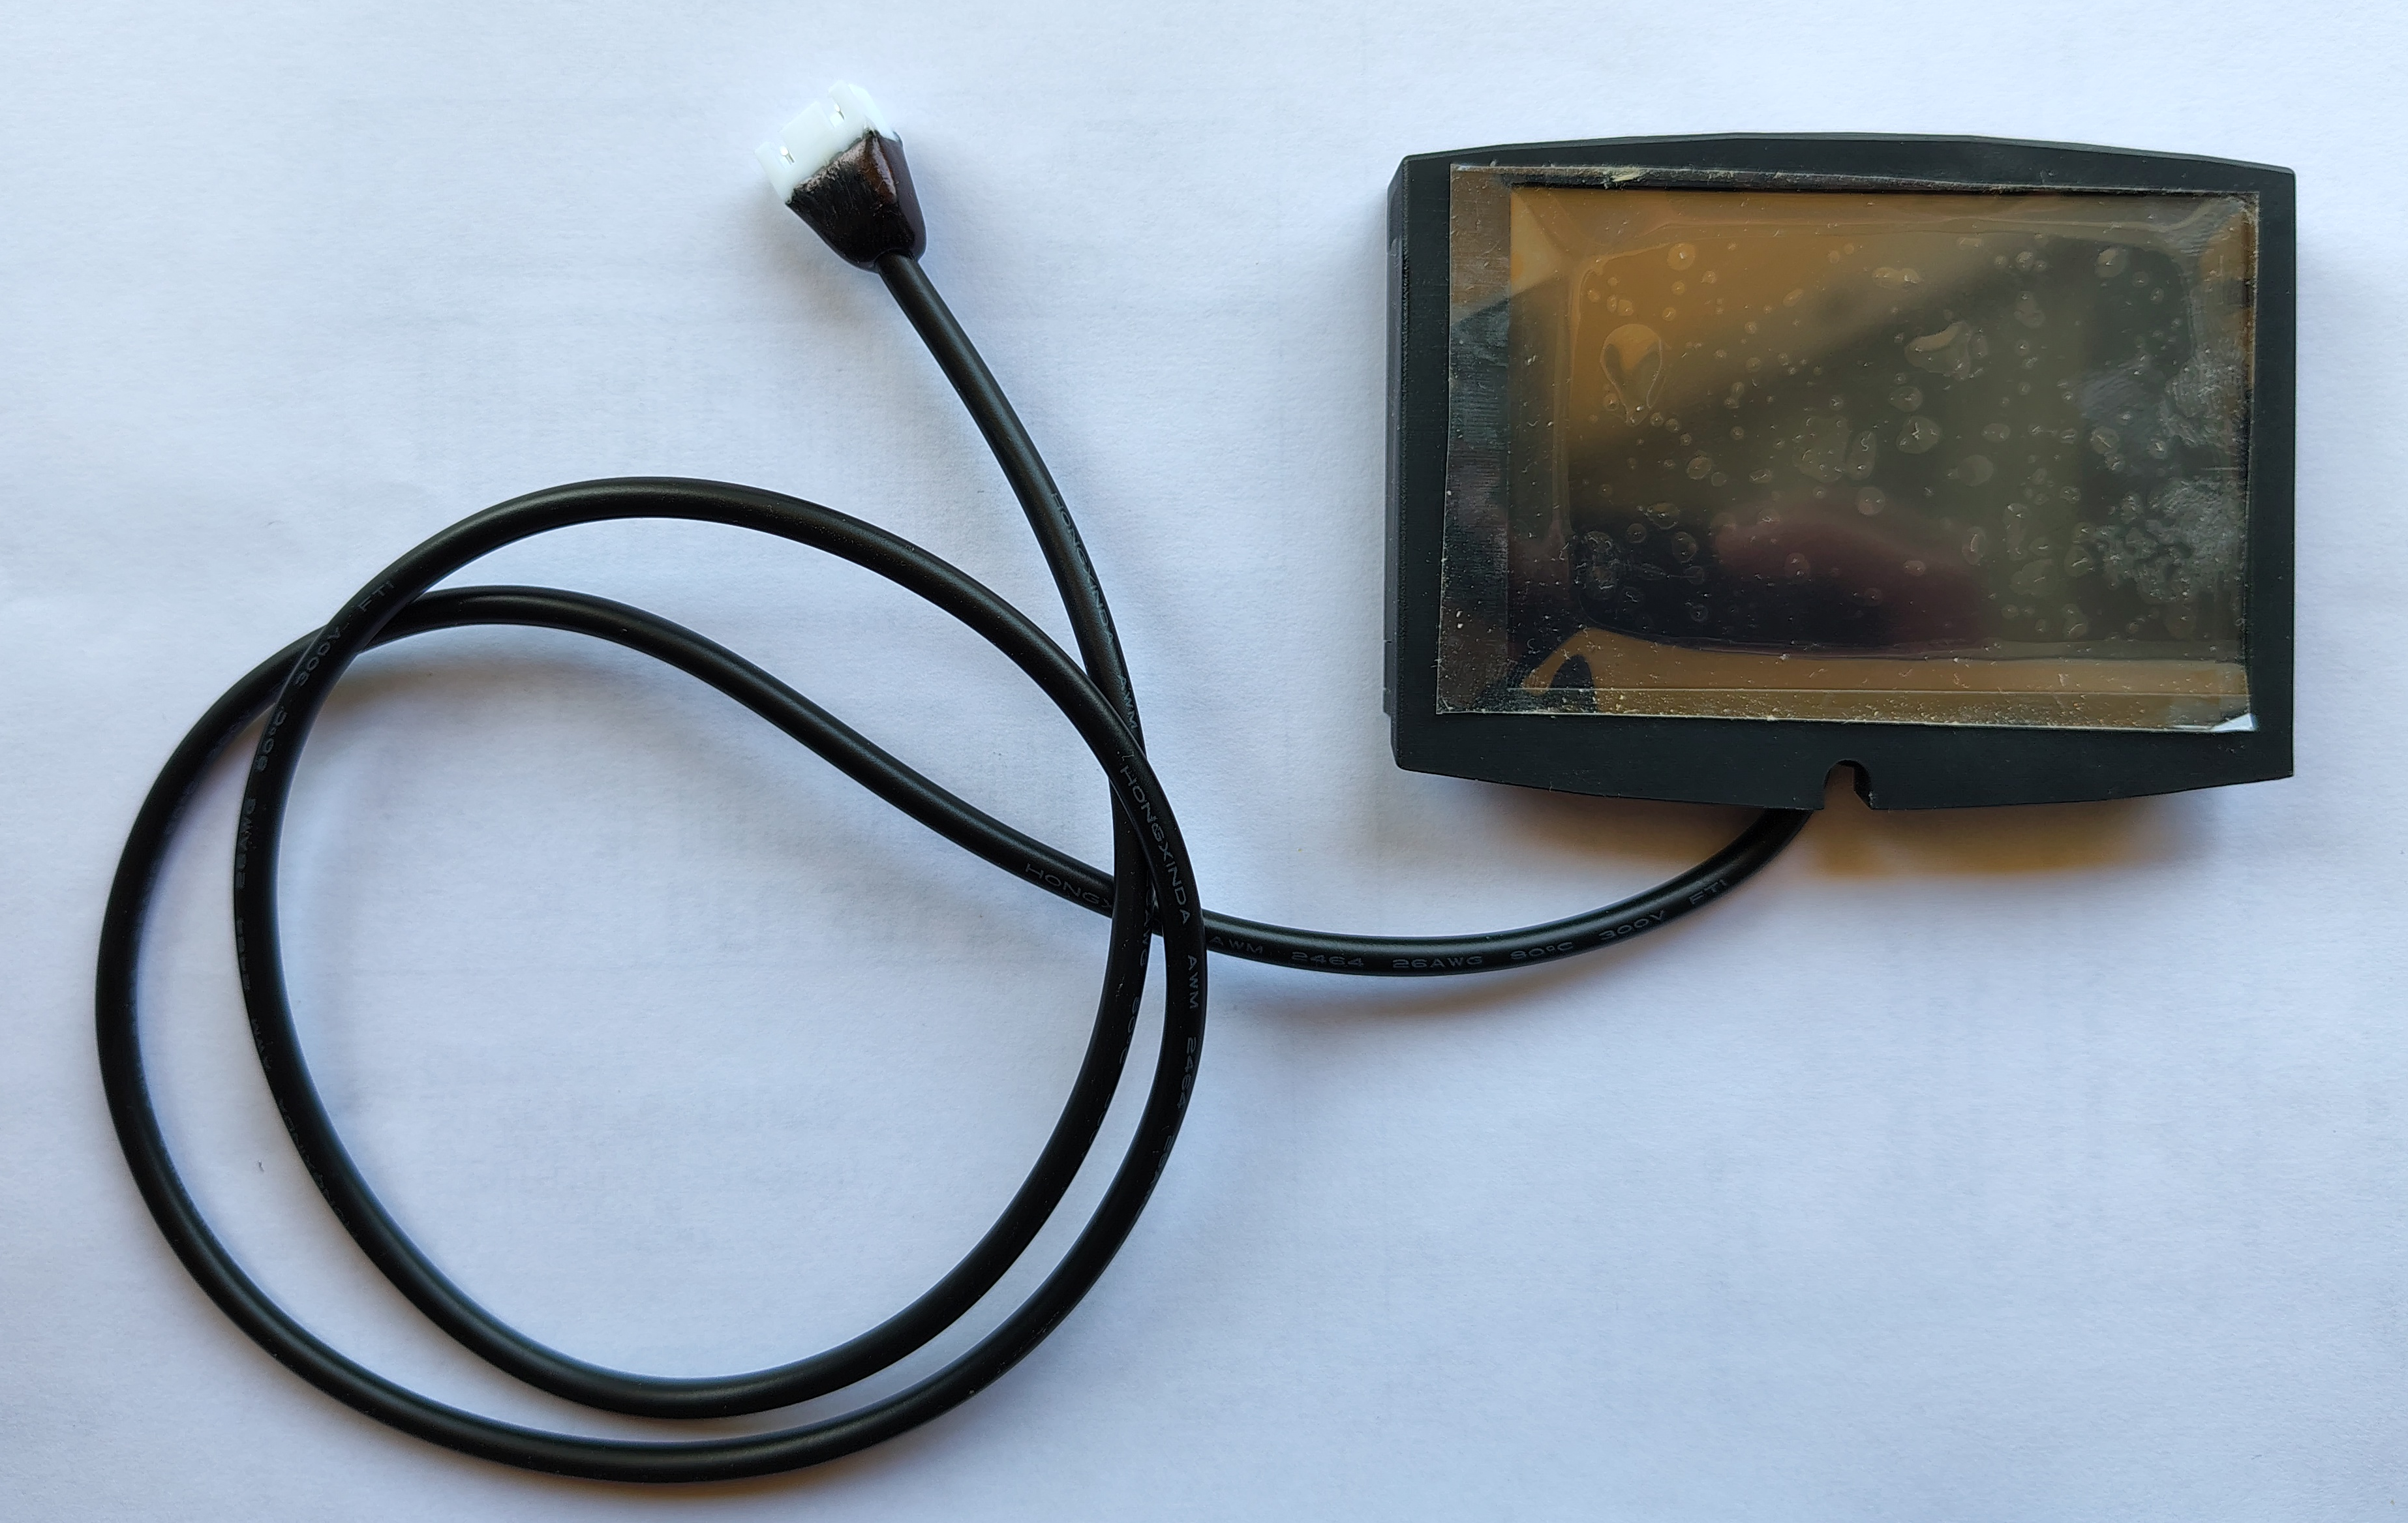
\includegraphics[width=0.8\textwidth]{figures/display.png}
    \caption{Écran LCD à clipser}
\end{figure}

L’écran, fourni avec un film de protection, comme le montrent les images, peut être placé dans le support imprimé en 3D afin de disposer d’un socle réglable que vous pouvez installer où vous le souhaitez.

\begin{figure}[H]
    \centering
    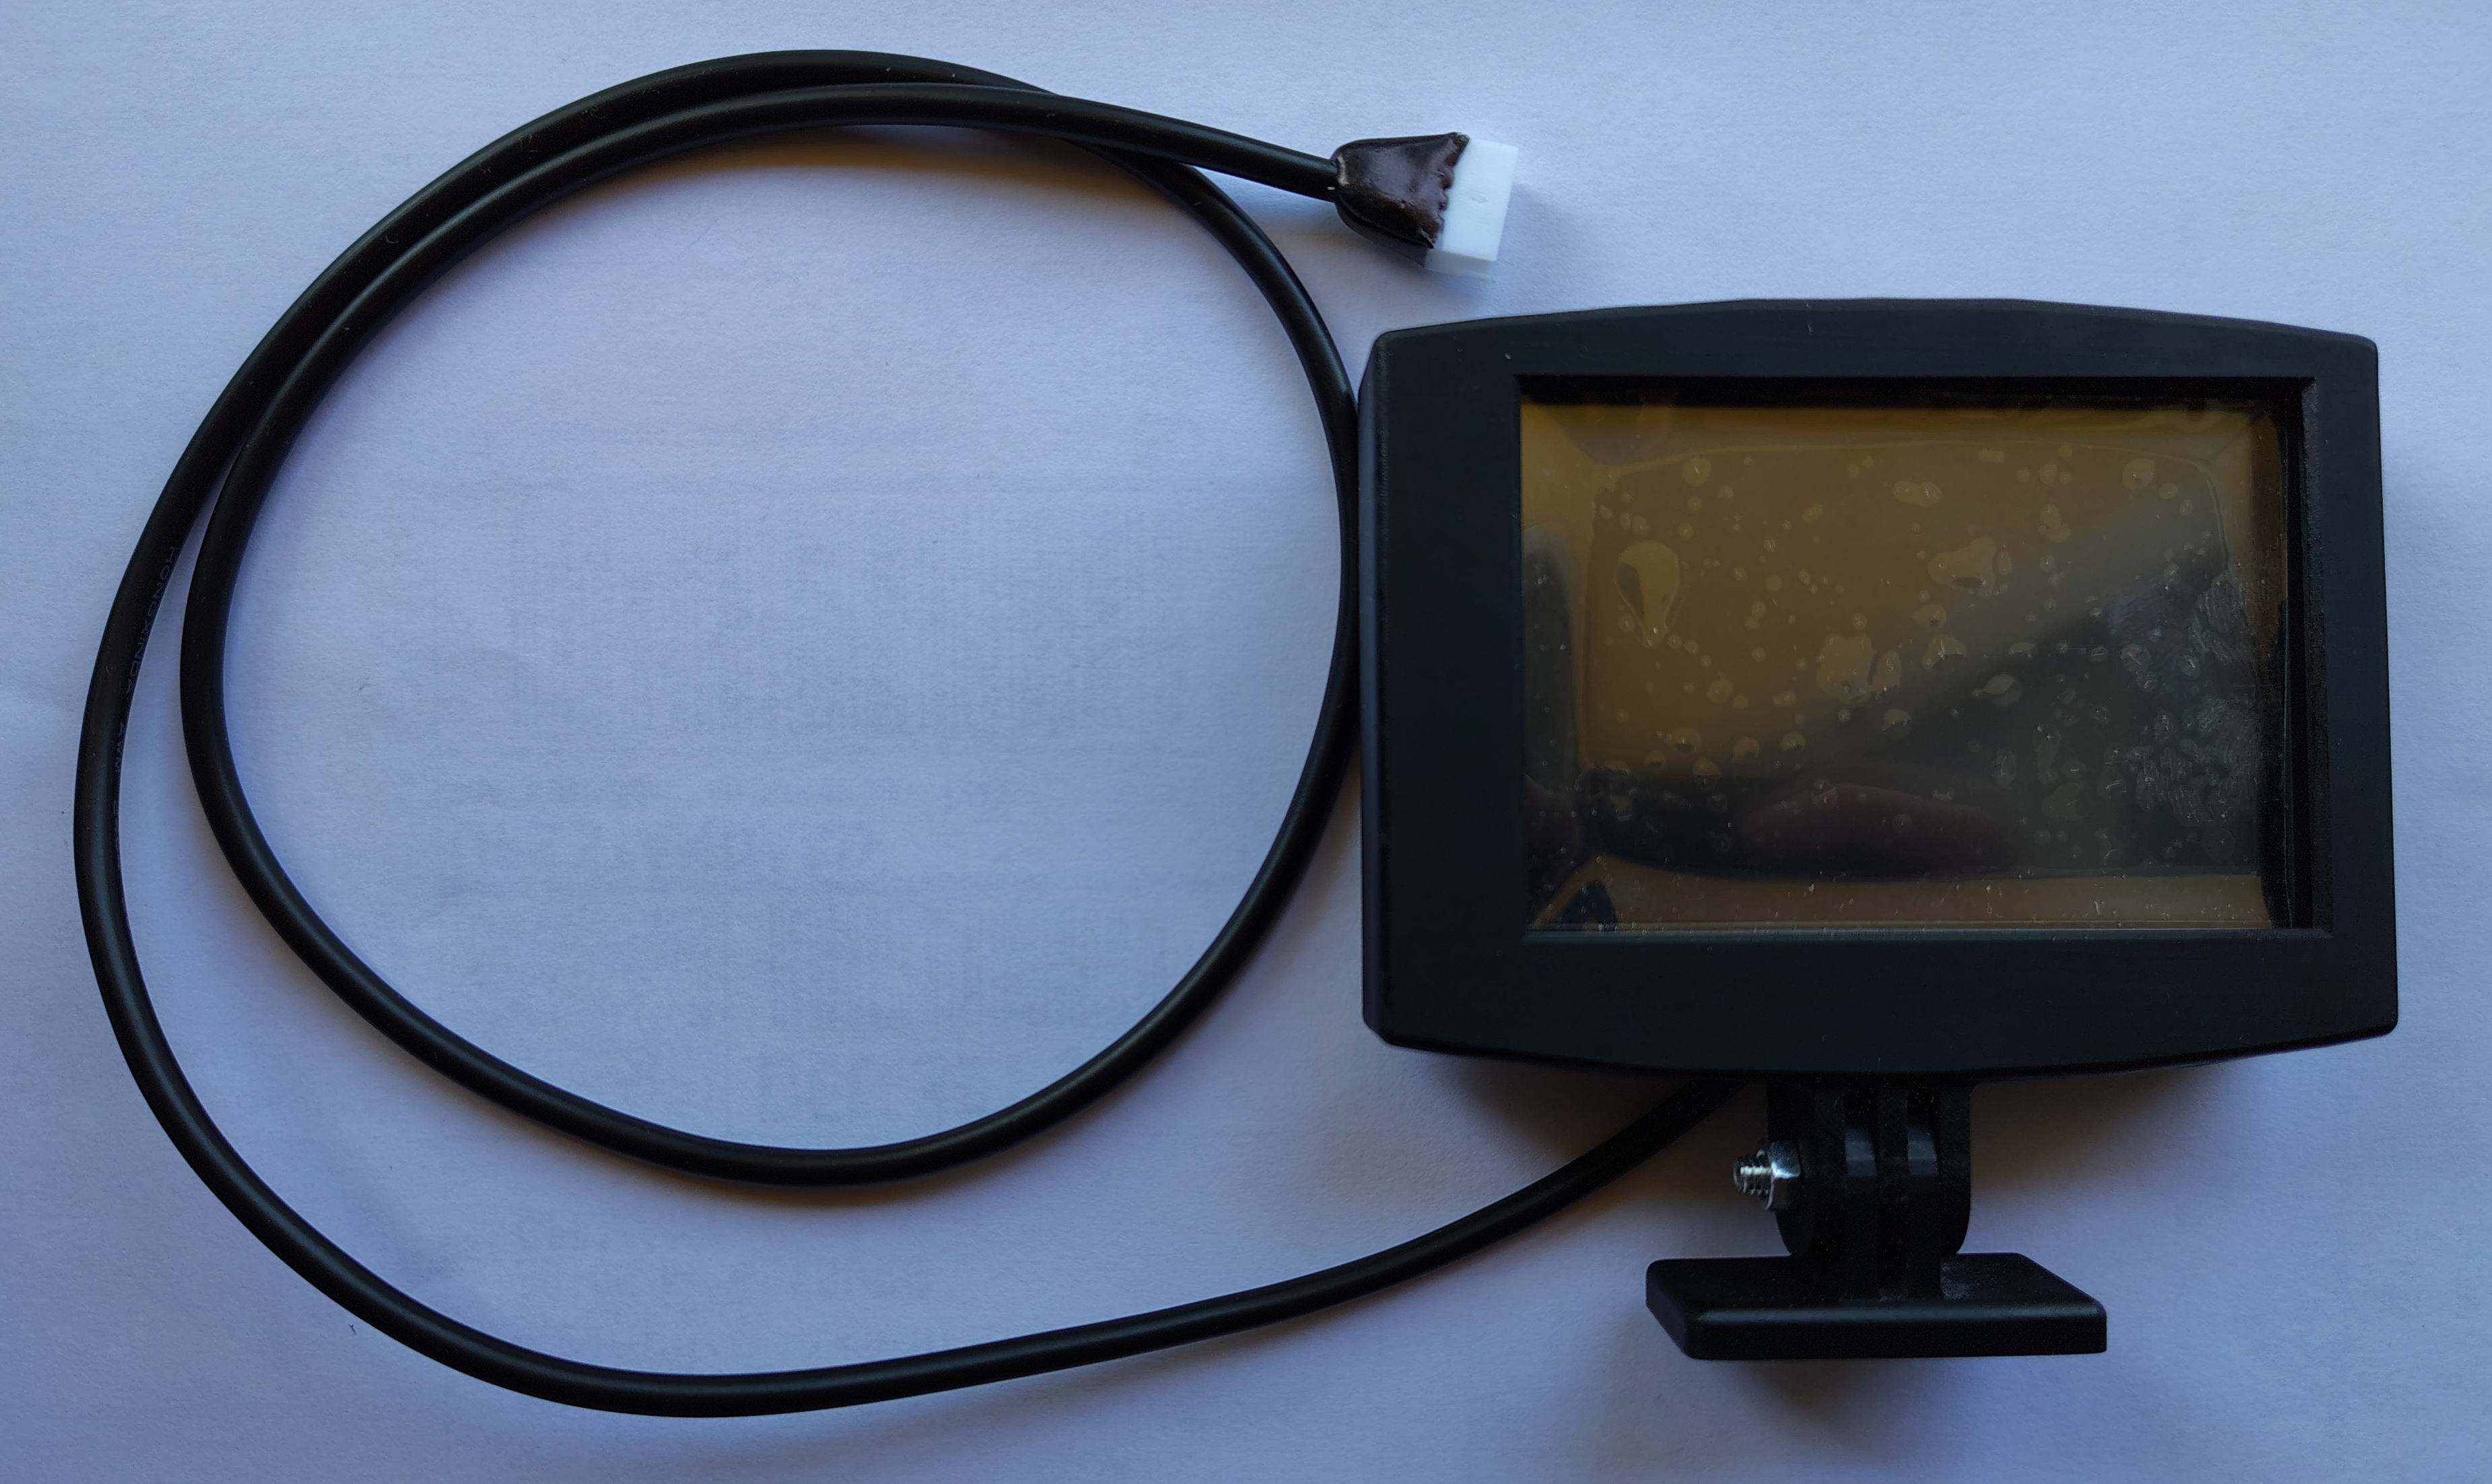
\includegraphics[width=0.8\textwidth]{figures/3d_stand_wdisplay.png}
    \caption{Écran LCD autonome}
\end{figure}

Dans la version autonome, vous pouvez le fixer à l’aide du cache et des vis fournis dans le colis, ainsi que du support pliable en 3D, comme le montrent les images ci-dessous.

\begin{figure}[H]
    \centering
    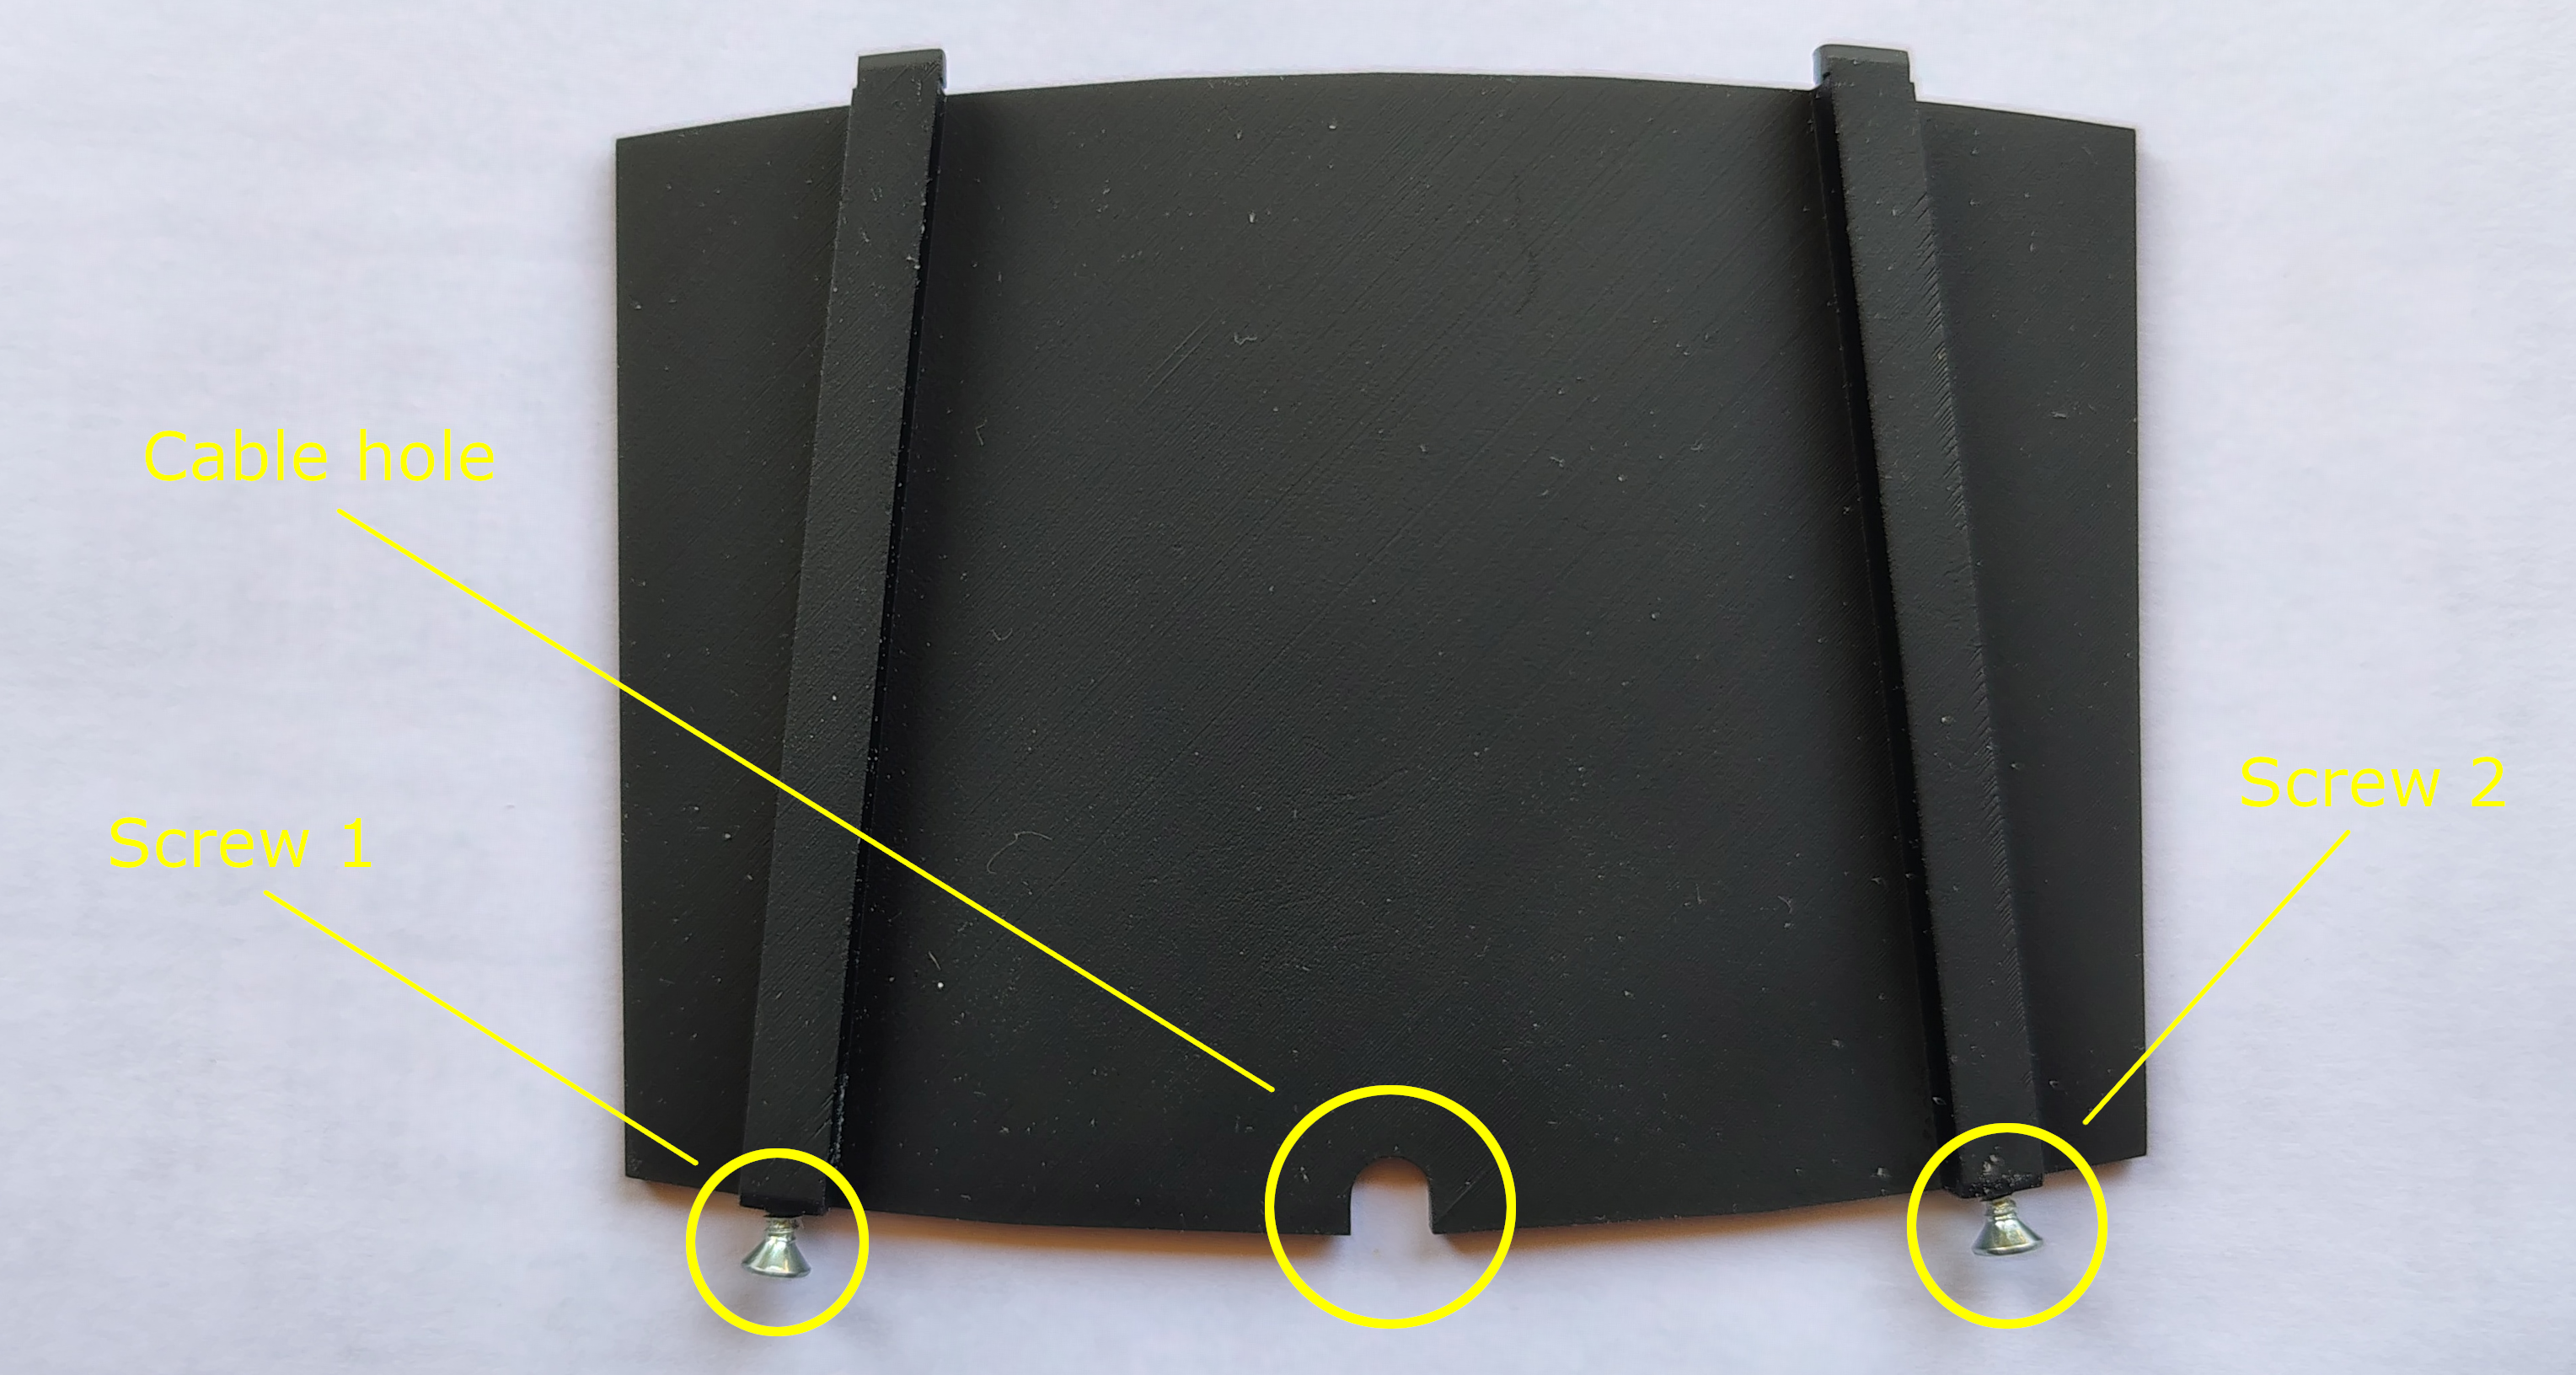
\includegraphics[width=0.8\textwidth]{figures/back_cover.png}
    \caption{Couvercle de l'écran LCD fourni}\label{fig:back_cover}
    \end{figure}

Le support 3D comporte également des trous sur sa base si vous souhaitez le visser sur la boîte à gants. Les autres trous sur le cadre sont destinés à visser le couvercle arrière afin de maintenir l'écran en place une fois à l'intérieur.

\begin{figure}[H]
    \centering
    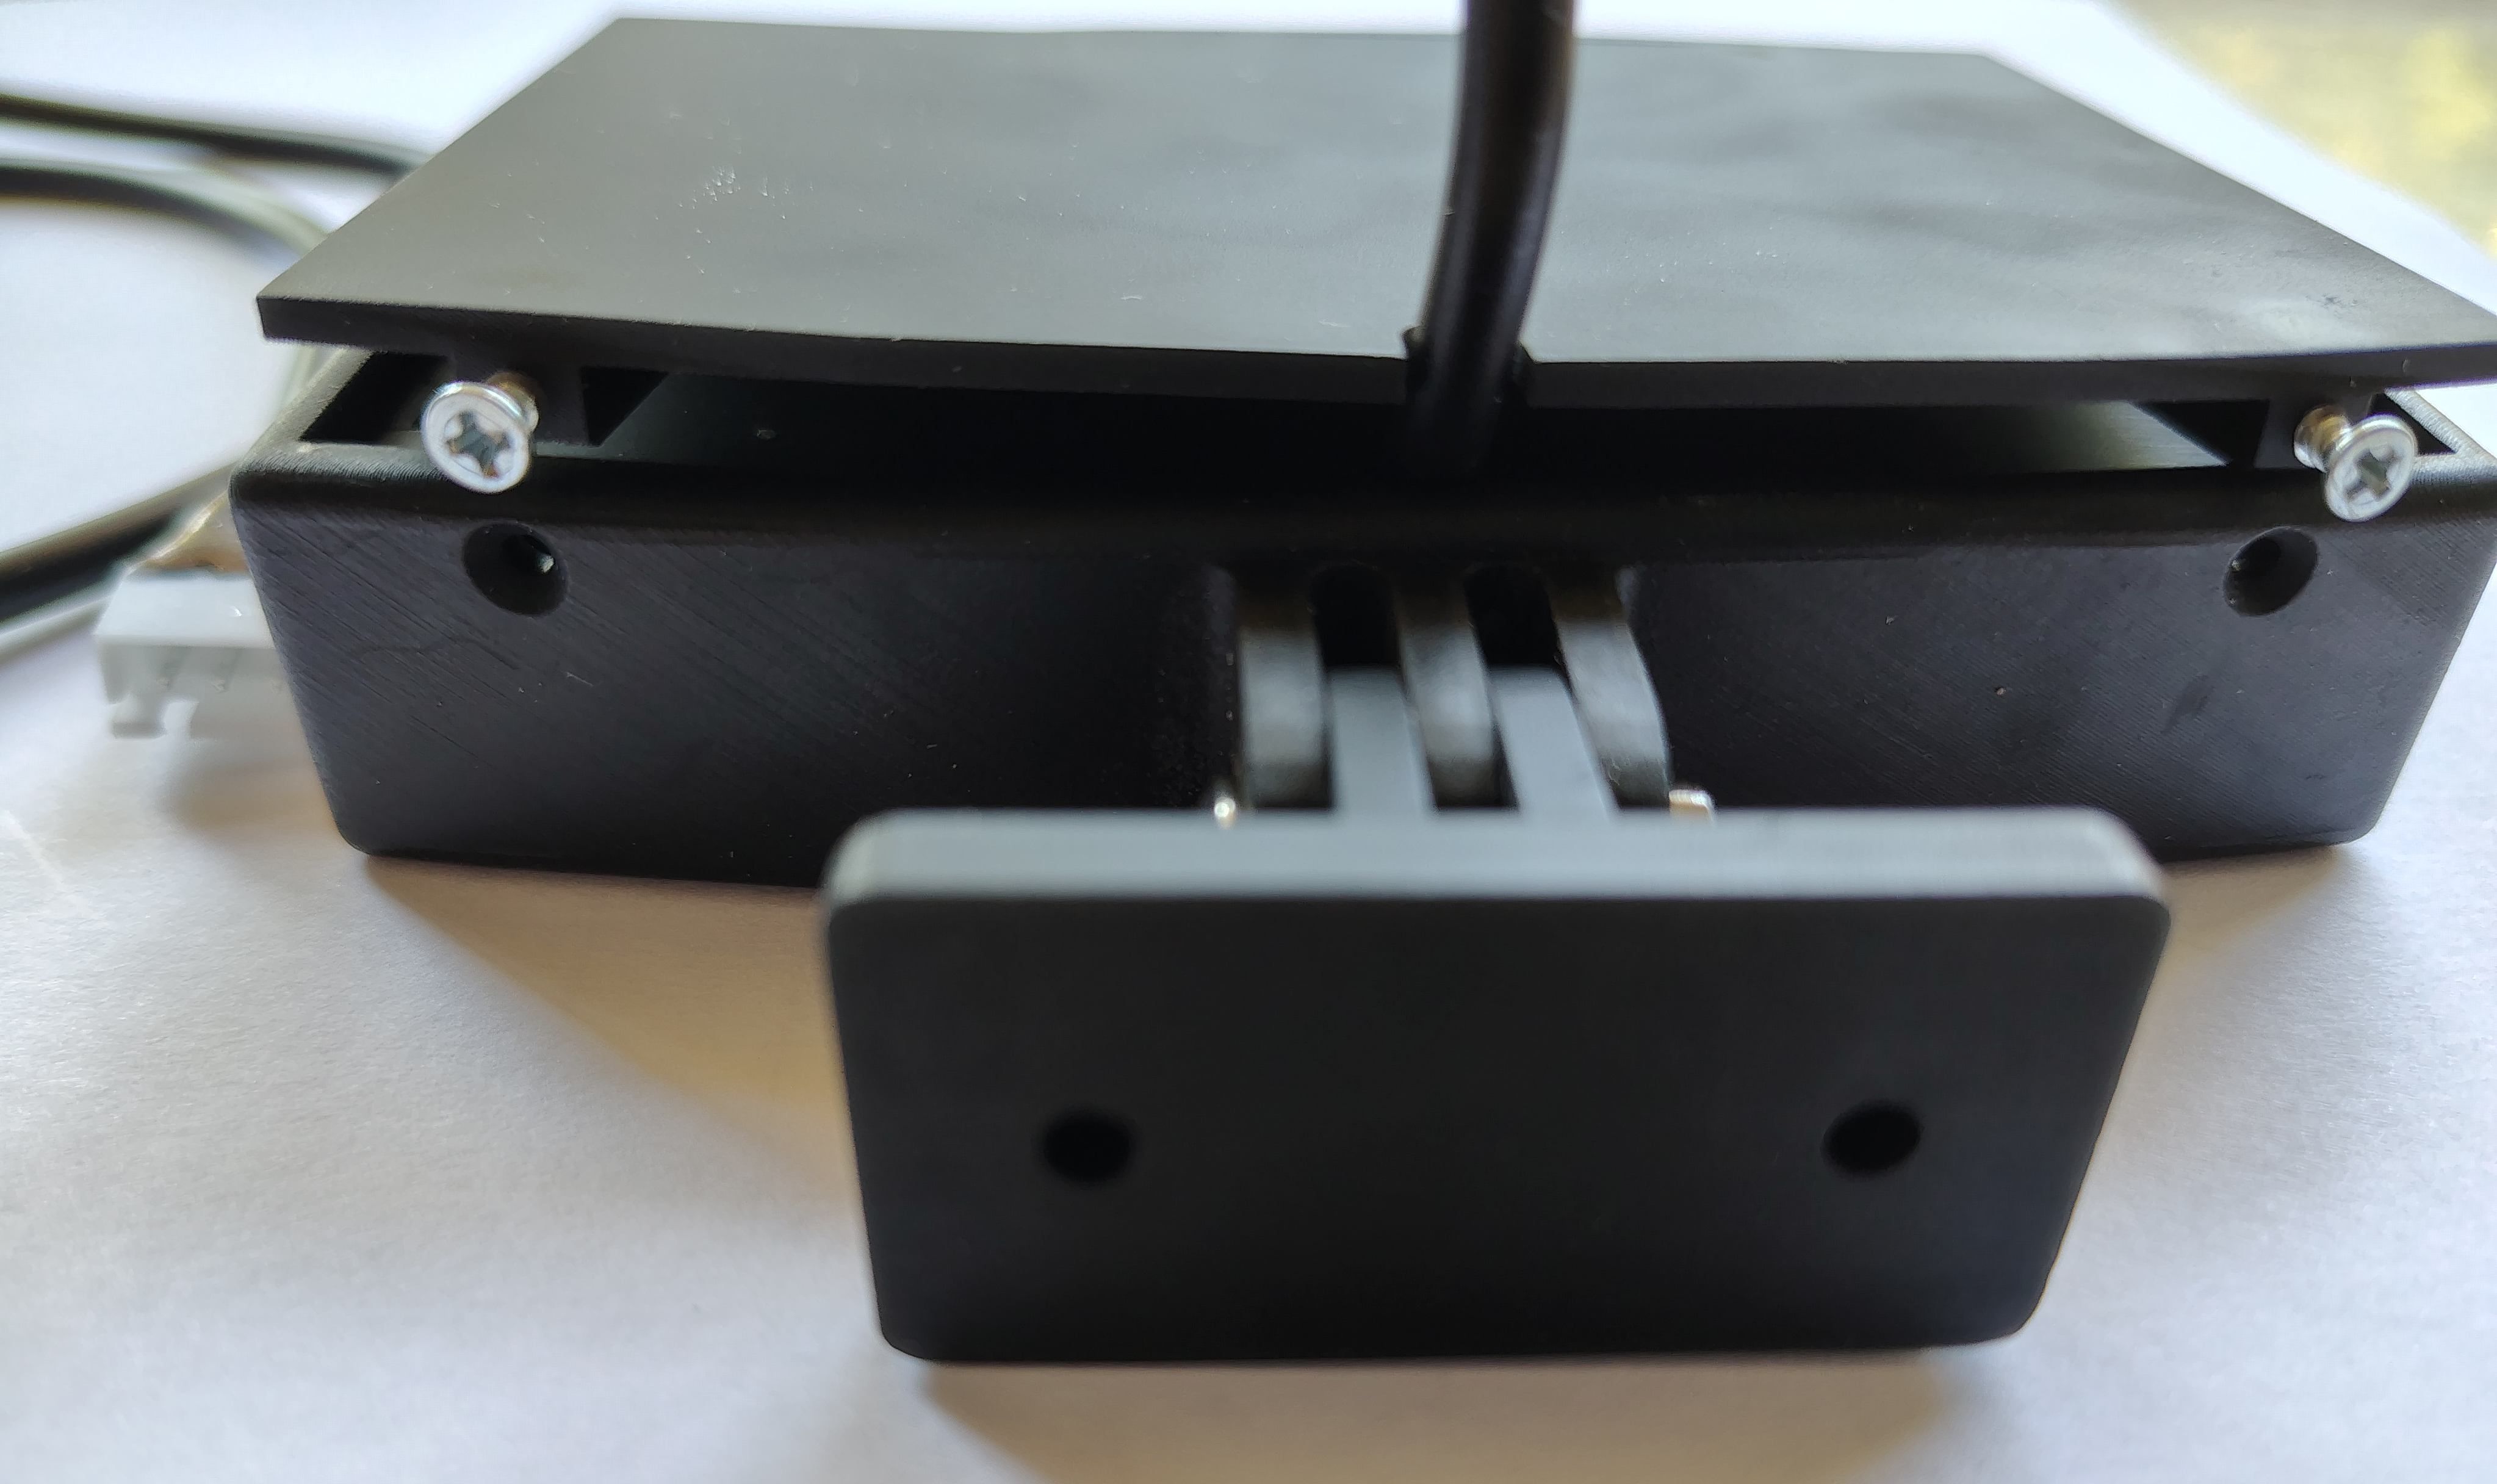
\includegraphics[width=0.8\textwidth]{figures/bottom_cover_screwholes.png}
    \caption{Fixation par vis du cache-écran LCD}\label{fig:bottom_cover_screwholes}
    \end{figure}

\subsection{Autres composants utiles}

Le kit comprend un serre-câble permettant de fixer le support imprimé en 3D pour le bouton sur la manette droite d’essuie-glace (également fournie). De plus, un autocollant est offert en bonus si vous souhaitez soutenir le projet en l'apposant quelque part sur votre Twizy.

\begin{figure}[H]
    \centering
    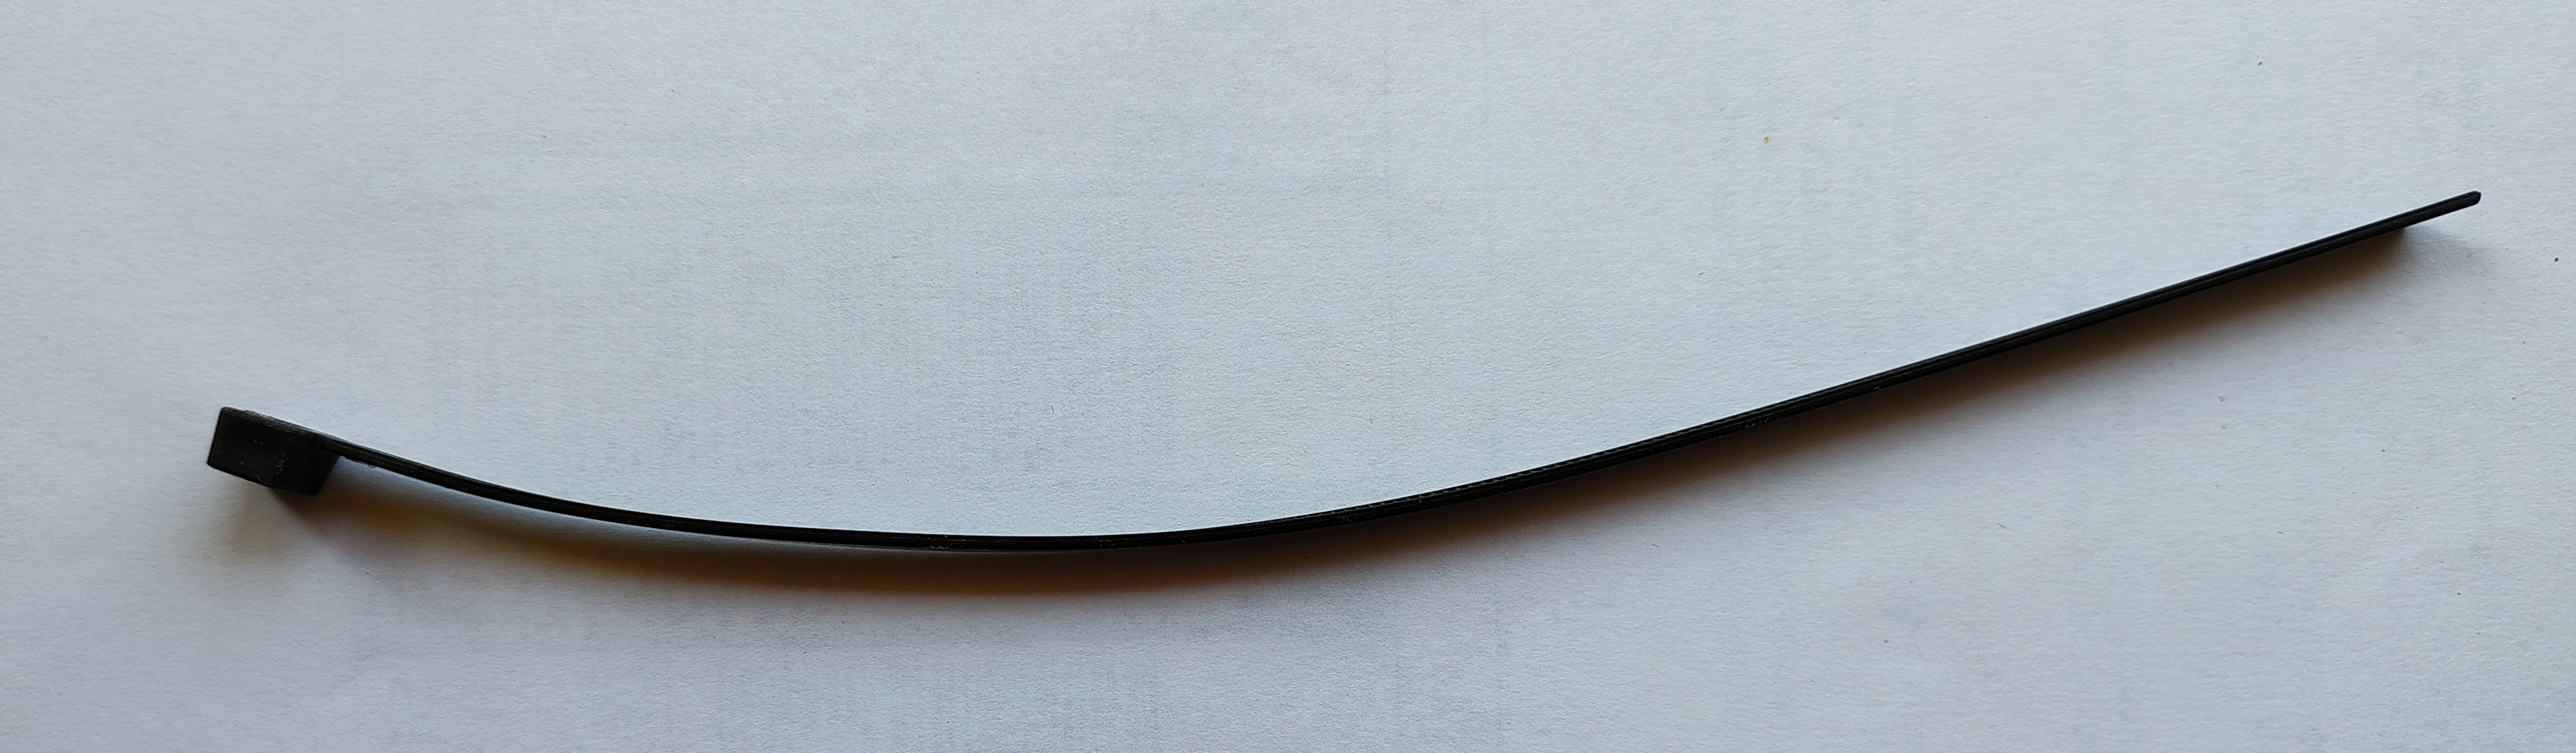
\includegraphics[width=0.8\textwidth]{figures/cable_tie.jpg}
    \caption{Attache-câble}\label{fig:cable_tie}
    \end{figure}

\begin{figure}[H]
    \centering
    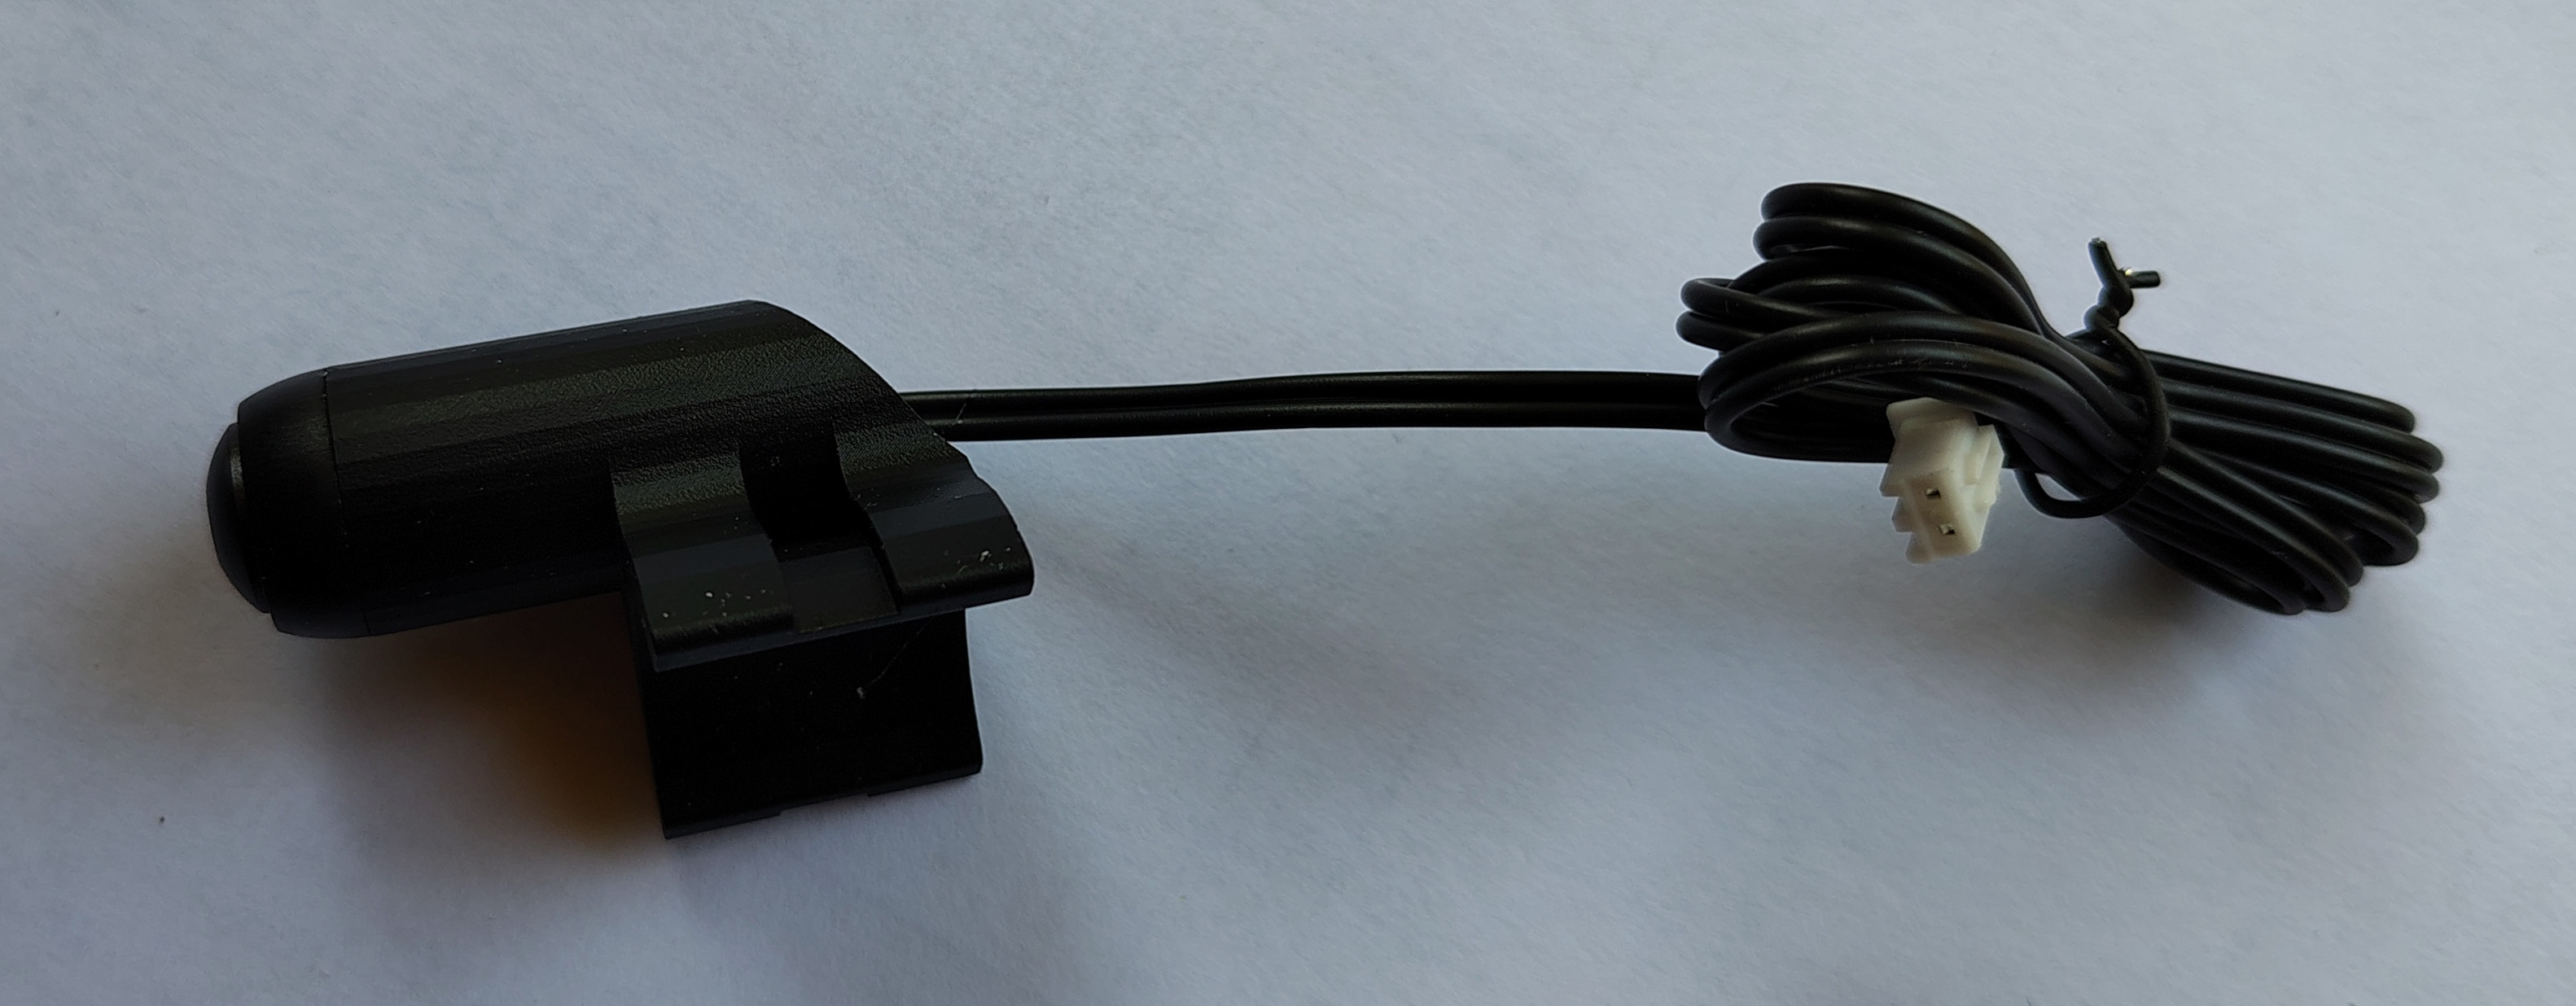
\includegraphics[width=0.8\textwidth]{figures/wiper_stalk_button.jpg}
    \caption{Bouton imprimé en 3D pour la manette d’essuie-glace}\label{fig:wiper_stalk_button}
    \end{figure}

\begin{figure}[H]
    \centering
    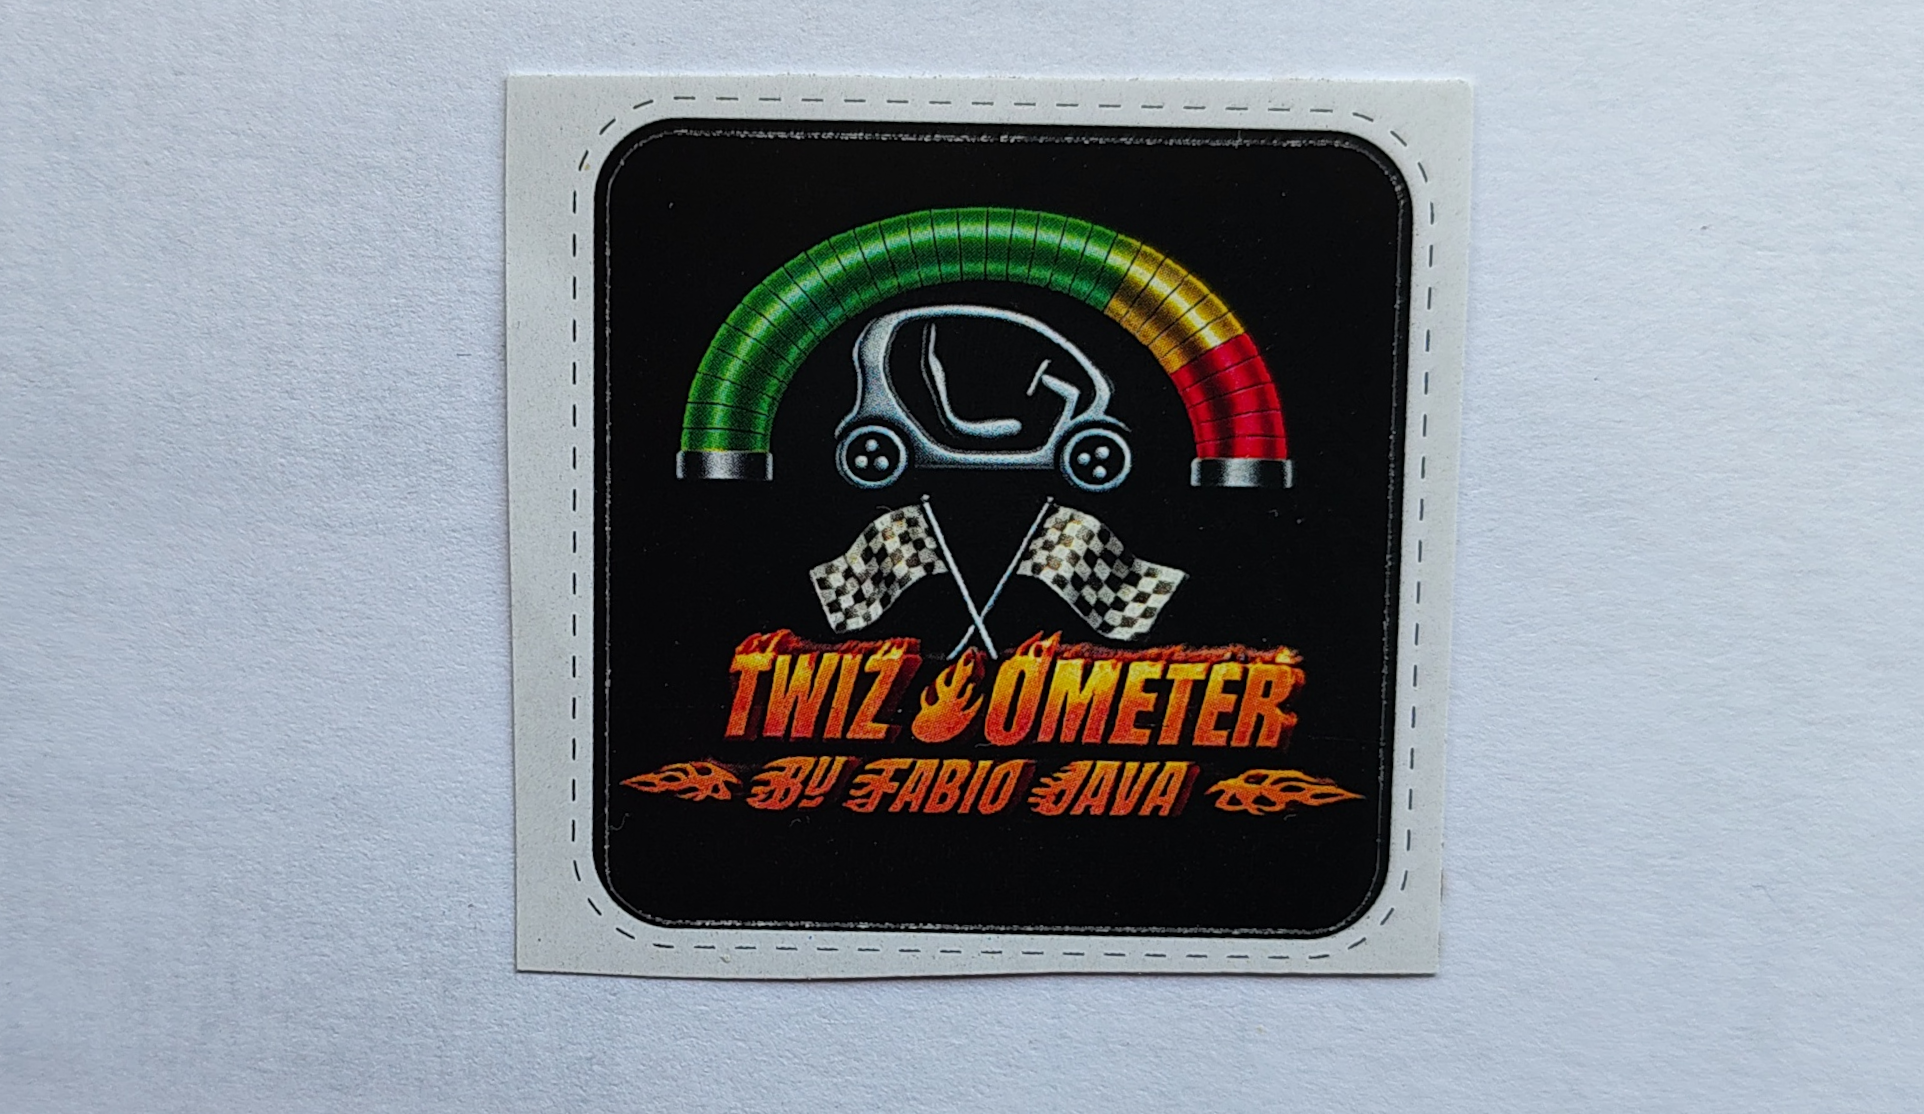
\includegraphics[width=0.8\textwidth]{figures/sticker.png}
    \caption{Autocollant ToM}
\end{figure}